\documentclass[a4paper]{article}
\usepackage[german,english]{babel}
\usepackage{amsmath}
\usepackage{amssymb}
\usepackage{amsthm}
\usepackage{graphicx}
\usepackage{caption}
\usepackage{fontspec}
\usepackage{mdframed}
\usepackage{pxfonts}
\usepackage{wasysym}
\usepackage{framed}
\usepackage{xcolor}
\usepackage{makeidx}
\usepackage{csquotes}
\usepackage[pdfborder={0 0 0}]{hyperref}
\usepackage{stmaryrd}
\usepackage{unicode-math}
\usepackage{titlesec}
\titleformat{\paragraph}{\normalfont\itshape}{}{}{}

% okay-ish main typefaces: Alegreya, Junicode, CMU Concrete, Linux Libertine O, Libertinus Serif, URW Palladio L, Bookerly, Andada
\setmainfont{Alegreya}
\setmathfont{cmr10}


\newcounter{lecref}[section]
\numberwithin{lecref}{section}

\theoremstyle{break}
\newmdtheoremenv[
    linecolor=white,%
    backgroundcolor=gray!10,%
    innertopmargin=0pt]{theorem}{Theorem}[lecref]

%\newtheorem{theorem}[lecref]{Theorem}
\newtheorem*{Theorem}{Theorem}
\newtheorem{example}[lecref]{Example}
\newtheorem*{Example}{Example}
\newtheorem{definition}[lecref]{Definition}
\newtheorem*{Definition}{Definition}
\newtheorem{lemma}[lecref]{Lemma}
\newtheorem*{Lemma}{Lemma}
\newtheorem{claim}[lecref]{Claim}
\newtheorem*{Claim}{Claim}
\newtheorem{remark}[lecref]{Remark}
\newtheorem*{Remark}{Remark}
\newtheorem{algorithm}{Algorithm}
\newtheorem*{Algorithm}{Algorithm}
\newtheorem{corollary}[lecref]{Corollary}
\newtheorem*{Corollary}{Corollary}
\newtheorem{proposition}[lecref]{Proposition}
\newtheorem*{Proposition}{Proposition}


\def\ifempty#1{\def\temp{#1} \ifx\temp\empty }

% chronological structure of lectures
\newcommand{\dateref}[1]{%
  \begin{mdframed}[backgroundcolor=gray!10,innerbottommargin=0pt,innertopmargin=0pt]
    \paragraph{\textit{$\downarrow$ This lecture took place on #1.}}%
  \end{mdframed}%
}

% useful control sequences for mathematical notation
\newcommand{\Abs}[1]{\left|#1\right|}
\newcommand{\Set}[1]{\left\{#1\right\}}
\newcommand{\SetDef}[2]{\left\{#1\,\mid\,#2\right\}}
\newcommand{\IP}[2]{\left\langle#1, #2\right\rangle}
\newcommand{\Norm}[1]{\left\|{\ifempty{#1}\cdot\else#1\fi}\right\|}
\newcommand{\Max}[1]{\max{\Set{#1}}}
\newcommand{\Min}[1]{\min{\Set{#1}}}
\newcommand{\Sup}[1]{\sup{\Set{#1}}}
\newcommand{\Powerset}[1]{{\mathbb P}(#1)}
\newcommand{\IntRange}[2]{#1, \dots\ifempty{#2}\else, #2\fi}

\def\vec2#1#2{\begin{pmatrix} #1 \\ #2 \end{pmatrix}}
\def\vec3#1#2#3{\begin{pmatrix} #1 \\ #2 \\ #3 \end{pmatrix}}
\newcommand{\noproof}[1]{A proof for Theorem~\ref{#1} is not provided.}
\newcommand{\dotted}[1]{\:\dot{#1}\:}  % dot has too little margin

% German translation
\newcommand{\dt}[1]{(dt. \enquote{\foreignlanguage{german}{#1}})}

% essential control sequences
%% \xRightarrow: \xrightarrow for \rightarrow like \xRightarrow for \Rightarrow
\makeatletter
\newcommand{\xRightarrow}[2][]{\ext@arrow 0359\Rightarrowfill@{#1}{#2}}
\makeatother

% typesetting settings
\parindent0pt
\setlength{\parskip}{.6em}

% TODO: span?
\DeclareMathOperator{\rank}{rank}
\DeclareMathOperator{\diag}{diag}
\DeclareMathOperator{\detm}{det}
\DeclareMathOperator{\perm}{perm}
\DeclareMathOperator{\sign}{sign}
\DeclareMathOperator{\degree}{deg}
\DeclareMathOperator{\im}{image}
\DeclareMathOperator{\ke}{kernel}
\DeclareMathOperator{\prop}{probability}
\DeclareMathOperator{\Hom}{Hom}
\DeclareMathOperator{\argmax}{argmax}
\DeclareMathOperator{\argmin}{argmin}
\DeclareMathOperator{\vol}{vol}  % volume
\DeclareMathOperator*{\bigtimes}{\vartimes}

% https://tex.stackexchange.com/a/110981, CC BY-SA
\makeatletter
\providecommand*{\dotcup}{%
  \mathbin{%
    \mathpalette\@dotcup{}%
  }%
}
\newcommand*{\@dotcup}[2]{%
  \ooalign{%
    $\m@th#1\cup$\cr
    \hidewidth$\m@th#1\cdot$\hidewidth
  }%
}
\makeatother

% metadata
\title{
  Computational Mathematics 1 \\
  \large{Lecture notes, University (of Technology) Graz} \\
  based on the lecture by Tobias Breiten
}
\date{\today}
\author{Lukas Prokop}

% generate index database
\makeindex

\begin{document}

\maketitle
\tableofcontents

\section*{Course}

\dateref{2018/10/02}

\begin{itemize}
  \item \href{https://imsc.uni-graz.at/breiten/teaching/numa18/}{Homepage at uni-graz.at}
  \item Contents:
    \begin{enumerate}
      \item Linear equation system
      \item Numerical error analysis
      \item Curve fitting~\dt{Lineare Ausgleichsrechnung}
      \item Non-linear equations
      \item Interpolation
      \item Numerical integration
    \end{enumerate}
  \item Literature:
    \begin{enumerate}
      \item Deuflhard, Hohmann: Numerische Mathematik 1
      \item Schwarz, Köckler: Numerische Mathematik
    \end{enumerate}
\end{itemize}

\clearpage
\section{What is Computational Mathematics?}
%
Computational Mathematics as branch of mathematics considers the construction and analysis of algorithms for continuous mathematical problems.
More specifically, based on a model and input data, we construct specific output data of interest.
Formally, we associate a model using function $f: X \to Y$ where $X$ is the set of input data and $Y$ the set of output data. The problem is to find output $f(x) \in Y$ for given $x \in X$.

Examples:
\begin{itemize}
  \item Addition of two numbers: $X = \mathbb R^2, Y = \mathbb R, f: (x_1, x_2) \mapsto x_1 + x_2$
  \item Solution of a linear equation system: $Ax = b$
    \[ X = \mathbb R^{n \times n} \times \mathbb R^n, Y = \mathbb R^n, f: (A, b) \mapsto A^{-1} b \]
\end{itemize}

An algorithm is defined as unambiguous sequence of steps to solve a given problem. A problem is characterized as
\begin{itemize}
  \item the input data required for computation
  \item the output data that represent the solution of the algorithm
  \item the description of the steps to be done, including auxiliary values
\end{itemize}
We require, the algorithm is
\begin{description}
  \item[executable] by a machine
  \item[terminating] after a finite number of steps
  \item[deterministic] as the same input always leads to the same output
\end{description}
Furthermore we analyze the algorithm in terms of
\begin{description}
  \item[stability] small errors in the input lead to small errors in the output
  \item[precision] output data should solve the problem with maximum accuracy
  \item[efficiency] large problems can be solved in practical time
\end{description}

Consider the linear equation system
\begin{align*}
  a_{11} x_1 + a_{12} x_2 + \dots + a_{1n} x_n &= b \\
  \vdots &= \vdots \\
  a_{n1} x_1 + a_{n2} x_2 + \dots + a_{nn} x_n &= b \\
\end{align*}
The same can be specified in compact notation like $Ax = b$ with $A \in \mathbb R^{n \times n}, b \in \mathbb R^n$.

\index{Cramer's rule}
\begin{theorem}[Cramer's Rule]
  Let $A \in \mathbb R^{n \times n}$ with $\det(A) \neq 0$ and $b \in \mathbb R^n$.
  Then there exists exactly one $x \in \mathbb R^n$ such that $Ax = b$. We can determine $x$ using \enquote{Cramer's Rule}:
  \[
    x_i = \frac{\det(A_i)}{\det(A)} \text{ where }
    A_i = \begin{bmatrix}
      a_{11} & \dots & a_{1, i-1} & b_1 & a_{1,i+1} & \dots & a_{1n} \\
      \vdots &       &            &     &           &       & \vdots \\
      a_{n1} & \dots & a_{n,i-1}  & b_n & a_{n,i+1} & \dots & a_{nn}
    \end{bmatrix}
  \]
\end{theorem}

\begin{Remark}[Problem]
  Computation using $\det(A) = \sum_{\sigma \in S_n} \sign(\sigma) a_{1,\sigma(1)} \dots a_{n,\sigma(n)}$ requires $n \cdot n!$ operations.
\end{Remark}

\subsection{Solving linear eq. system by forward/backwards substitution}
%
Consider the special case of a linear equation system of structure
\[
  \begin{array}{rrrrl}
    \gamma_{11} x_1 &+ \gamma_{12} x_2 &+ \dots &+ \gamma_{1n} x_n &= z_1 \\
                    &  \gamma_{22} x_2 &+ \dots &+ \gamma_{2n} x_n &= z_2 \\
                    &                  & \ddots &                  &= \vdots \\
                    &                  &        &  \gamma_{nn} x_n &= z_n
  \end{array}
\]%
\index{Backwards substitution}%
and accordingly, $Rx = z$ with an upper triangular matrix, hence $\gamma_{ij} = 0$ for $i > j$.
We retrieve $x$ by recursive solution (by so-called \enquote{backwards substitution}) starting with row $n$:
\begin{align*}
  x_n &= \frac{z_n}{\gamma_{nn}} \text{ if } \gamma_{nn} \neq 0 \\
  x_{n-1} &= \frac{z_{n-1} - \gamma_{n-1,n} x_n}{\gamma_{n-1,n-1}} &\text{ if } \gamma_{n-1,n-1} \neq 0 \\
  x_{1} &= \frac{z_1 - \gamma_{12} x_2 - \dots - \gamma_{1n} x_n}{\gamma_{11}} &\text{ if } \gamma_{11} \neq 0
\end{align*}

Obviously, it holds that
\[ \det(R) = \gamma_{11} \dots \gamma_{nn} \neq 0 \iff \gamma_{ii} \neq 0 \qquad \forall i = 1, \dots, n \]
The algorithm is applicable (just like Cramer's rule), if $\det(R) \neq 0$.
Then the existence of a solution is guaranteed and this solution is unique.

\begin{Remark}[Computing time]\hfill{}
  \begin{enumerate}
    \item for the $i$-th row, we need $(n-i)$ additions, $(n-i)$ multiplications and one division
    \item in total for the rows $n$ to $1$,
      \[ \sum_{i=1}^n (i - 1) = \frac{n (n - 1)}2 \dotted{=} \frac{n^2}2 \]
      Multiplication and the same amount of additions.
      The notation $\dot=$ is used to denote equivalence up to terms of same degree.
      Analogously, the equation system $Lx = z$ can be solved with a lower triangular matrix $L$ by forward substitution starting with the first row.
  \end{enumerate}
\end{Remark}

\subsection{Gaussian elimination process} % 1.2

\emph{Basic idea:}
\begin{quote}
  Beginning with a linear equation system of structure,
  \begin{align}
    a_{11} x_1 + a_{12} x_2 + \dots + a_{1n} x_n &= b_1 \nonumber\\
    a_{21} x_1 + a_{22} x_2 + \dots + a_{2n} x_n &= b_2 \nonumber\\
    \vdots &= \vdots \nonumber\\
    a_{n1} x_1 + a_{n2} x_2 + \dots + a_{nn} x_n &= b_n
    \label{eq1}
  \end{align}
  we apply equivalence transformations to end up with an upper triangular matrix.
\end{quote}

As a first step, we eliminate variable $x_1$ of rows $2$ to $n$.
\begin{align}
  a_{11} x_1 + a_{12} x_2 + \dots + a_{1n} x_n &= b_1 \nonumber\\
    a_{22}' x_2 + \dots + a_{2n}' x_n &= b_1 \nonumber\\
      \vdots &= \vdots \nonumber\\
      a_{12}' x_2 + \dots + a_{nn}' x_n &= b_n'
  \label{eq2}
\end{align}
So we apply this elimination step ($r_i \coloneqq \frac{r_i}{a_{i1}} - \frac{r_1}{a_{11}}$ where $r_i$ denotes the $i$-th row) to the last $n-1$ rows and determine the triangular matrix recursively this way.

Consider the transformation of~\eqref{eq1} to \eqref{eq2}.
Let $a_{11} \neq 0$ and we recognize $\text{row}_i \coloneqq \text{row}_i - l_{i_1} \cdot \text{row}_1$.
Formally,
\[ \underbrace{(a_{i1} - l_{i1} a_{11}) x_1}_{=0} + \underbrace{(a_{i2} - l_{i1} a_{12})}_{a_{i2}'} x_2 + \dots + \underbrace{(a_{in} - l_{i1} a_{1n})}_{a_{in}'} x_n = \underbrace{b_i - l_{in} b_1}_{b_i'} \]
\[ \implies l_{in} = \frac{a_{i1}}{a_{11}} \]
hence, the first elimination step is applicable if $a_{11} \neq 0$ is given.
If we apply this step, we retrieve a sequence of matrices:
\[ A = A^{(1)} \to A^{(2)} \to \dots \to A^{(n)} = R \]
where
\[
  A^{(k)} = \begin{bmatrix}
    a_{11}^{(1)} & a_{12}^{(1)} & \dots  &              &        & a_{1n}^{(1)} \\
    0            & a_{22}^{(2)} & \dots  &              &        & a_{2n}^{(2)} \\
                 &              & \ddots &              &        & \vdots \\
                 &              &        & a_{kk}^{(k)} & \dots  & a_{kn}^{(k)} \\
                 &              &        & \vdots       &        & \vdots \\
                 &              &        & a_{nk}^{(k)} & \dots  & a_{nn}^{(k)}
  \end{bmatrix}
\]
with a remaining matrix of dimension $(n - k + 1) \times (n - k + 1)$.
For every remaining matrix we can apply the elimination step
\begin{align*}
  l_{ik} &= \frac{a_{ik}^{(k)}}{a_{kk}^{(k)}} &\text{ for } i = k+1, \dots, n \\
  a_{ij}^{(k+1)} &= a_{ij}^{(k)} - l_{ik} a_{kj}^{(k)} &\text{ for } i,j = k+1, \dots, n \\
  b_i^{(k+1)} &= b_i^{(k)} - l_{ik} b_k^{(k)} &\text{ for } i = k+1, \dots, n
\end{align*}
under the assumption that $a_{kk}^{(k)} \neq 0$ (pivot element).

\index{Frobenius matrix}
\begin{Remark}
  Every elimination step is a linear operation of the rows of $A$.
  Hence it is representable by left multiplication with $L_k \in \mathbb R^{n \times n}$ according to $A^{k+1} = L_k A^{(k)}$ and $b^{(k+1)} = L_k b^{(k)}$.

  The following matrix is a \emph{Frobenius matrix}, which has an interesting property regarding its inverse:
  \index{Frobenius matrix}
  \[
    L_k = \begin{pmatrix}
      1 &        &   &                 &        & \\
        & \ddots &   &                 &        & \\ 
        &        & 1 &                 &        & \\
        &        & -l_{k+1,k} & \ddots &        & \\
        &        & \vdots     &        & \ddots & \\
        &        & -l_{n,k}   & \dots  &        & 1
    \end{pmatrix}
    \iff
    L_k^{-1} = \begin{pmatrix}
      1 &        &   &                 &        & \\
        & \ddots &   &                 &        & \\ 
        &        & 1 &                 &        & \\
        &        & l_{k+1,k}  & \ddots &        & \\
        &        & \vdots     &        & \ddots & \\
        &        & l_{n,k}    & \dots  &        & 1
    \end{pmatrix}
  \]
\end{Remark}
and
\[
  L = L_1^{-1} \quad \dots \quad L_{n-1}^{-1} =
  \begin{pmatrix}
    1      &        &        &           & 0 \\
    l_{21} & \ddots &        &           & \\
    l_{31} & l_{32} & \ddots &           & \\
    \vdots & \vdots &        &           & \\
    l_{n1} & \dots  &        & l_{n,n-1} & 1
  \end{pmatrix}
\] \[
  L^{-1} = L_{n-1} \dots L_1
\]

\index{LR decomposition}
This way, we retrieve an equivalent linear equation system to $Rx = z, R = L^{-1} A, z = L^{-1} b$.
The representation $A = LR$ is called \emph{LR decomposition of $A$}.
If they exists, $L$ and $R$ are unambiguously determined.
\[
  A = L_1 R_1 = L_2 R_2
  \implies R_1 = L_1^{-1} L_2 R_2
  \implies R_1 R_2^{-1} = L_1^{-1} L_2
\] \[
  \implies \text{ diagonal representation of } L_1^{-1} L_2 \dots, R_1 R_2^{-1}
\]

\begin{algorithm}[Gaussian elimination]\hfill{} % Algorithmus 1
  \begin{enumerate}
    \item $A = LR$ with $R$ as upper triangular matrix, $L$ as lower triangular matrix
    \item Solve $Lz = b$ by forward substitution
    \item Solve $Rx = z$ by backwards substitution
  \end{enumerate}
  The entries $l_{ik} \neq 1$ can be stored in the remaining null-entries of the matrix $A^{(k)}$.
  Thus the total memory requirements are bounded by $n (n+1)$.
\end{algorithm}

\begin{Remark}[Computing time]\hfill{}
  \begin{itemize}
    \item $\sum_{k=1}^{n-1} k^2 \dotted{=} \frac{n^3}{3}$ for step 1
    \item $\sum_{k=1}^{n-1} k \dotted{=} \frac{n^2}{2}$ for step 2 and 3
  \end{itemize}
\end{Remark}

\subsection{Pivot strategies}

\textbf{Problem:} The algorithm above does not work for the simple example:
\[ A = \begin{bmatrix} 0 & 1 \\ 1 & 0 \end{bmatrix} \qquad \det(A) = -1 \neq 0 \]
We \emph{need} row exchanges.
We can evaluate, that no LU-decomposition exists.

But exchange of the rows gives
\[
  A = \begin{bmatrix} 0 & 1 \\ 1 & 0 \end{bmatrix}
  \leadsto \hat{A} = \begin{bmatrix} 1 & 0 \\ 0 & 1 \end{bmatrix}
  = I = LU
\]
with $L = U = I$.

\begin{example} % Beispiel 1.2
  Consider the equation system
  \begin{align*}
    1 \cdot 10^{-4} x_1 + 1 \cdot x_2 &= 1 \\
    1 \cdot x_1 + 1 \cdot x_2 &= 2
  \end{align*}
  \textbf{Assumption:} Compute up to three decimal points.
  Then for the \enquote{accurate} solution, we get $x_1 = 1$ and $x_2 = 1$.
\end{example}

Using the Gaussian elimination process, we get
\[ l_{21} = \frac{a_{21}}{a_{11}} = 10^4 \]
\[ \implies 0 \cdot x_1 + (1 - 10^4 \cdot 1) x_2 = 2 \cdot 10^4 \cdot 1 \]
Therefore we get the triangular system
\[ 10^{-4} x_1 + 1 \cdot x_2 = 1 \]
\[ -10^4 x_2 = -10^4 \]
By this, we get an approximation $x_2 = 1$ and $x_1 = 0$.

In contrast, if we exchange the two rows,
\begin{align*}
  1 \cdot x_1 + 1 \cdot x_2 &= 2 \\
  10^{-4} x_1 + 1 \cdot x_2 &= 1
\end{align*}
then $\tilde{l}_21 = \frac{10^4}{1}$ follows and therefore the triangular system
\begin{align*}
  1 \cdot x_1 + 1 \cdot x_2 &= 2 \\
  1 \cdot x_2 &= 1
\end{align*}
with the \enquote{correct} solution is $x_2 = 1$ and $x_1 = 1$.

Our exchange of the rows has given us $\Abs{\tilde{l}_{21}} < 1$ and $\Abs{\tilde{a}_{11}} \geq \Abs{\tilde{a}_{21}}$.

\dateref{2018/10/04}
The new pivot element $\tilde{a}_{11}$ is the largest absolute value in the first column.
Thus, we apply the column pivot strategy: In every step, choose the row with the largest, absolute value in the pivot column.

\begin{algorithm}[Gaussian elimination with column pivot strategy]\hfill{}
  \label{algo2}
  \begin{enumerate}
    \item In step $A^{(k)} \to A^{(k+1)}$, choose some $p \in \Set{k, \dots, n}$ such that $\Abs{a_{p_k}^{(k)}} \geq \Abs{a_{jk}^{(k)}}$ for $j = k, \dots, n$
    \item Exchange rows $p$ and $k$
      \[
        A^{(k)} \leadsto \tilde{A}^{(k)} \text{ with } \tilde{a}_{ij}^{(k)}
        = \begin{cases}
          a_{kj}^{(k)} & i = p \\
          a_{pj}^{(k)} & i = k \\
          a_{ij}^{(k)} & \text{else}
        \end{cases}
      \]
    \item Apply the elimination step $\tilde{A}^{(k)} \to \tilde{A}^{(k+1)}$
  \end{enumerate}
\end{algorithm}

\begin{remark} % Bemerkung 1.3
  We can apply the row pivot strategy with column exchange
  instead of the column pivot strategy with row exchange.
\end{remark}

\index{Permutation matrix}
We use permutation matrices $P \in \mathbb R^{n \times n}$ to analyze the column pivot search.
By permutation $\pi \in S_n$, we associate the \emph{permutation matrix}
\[ P_\pi = [e_{\pi(1)}, e_{\pi(2)}, \dots, e_{\pi(n)}] \]
where $e_j$ denotes the $j$-th unit vector in $\mathbb R^n$. Row and column exchanges of a matrix $A$ can followingly be represented as
\[ \pi_z: A \mapsto P_{\pi} A, \qquad \pi_S: A \mapsto A P_{\pi} \]

\begin{Remark}
  It holds that $\det(P_{\pi}) = \sign(\pi) \in \Set{\pm 1}$ and $P_{\pi}^{-1} = P_{\pi}^{T}$.
  [Consider $P_\pi = e_{\pi(1)} \cdot e_1^T + e_{\pi(2)} e_2^T + \dots + e_{\pi(n)} e_n^T$.]
  \begin{align*}
    P_{\pi}^T &= e_1 e_{\pi(1)}^T + e_2 e_{\pi(2)}^T + \dots + e_n e_{\pi(n)}^T \\
    P_{\pi} P_{\pi}^T &= e_{\pi(1)} e_{\pi(1)}^T + e_{\pi(2)} e_{\pi(2)}^T + \dots + e_{\pi(n)} e_{\pi(n)}^T
  \end{align*}
\end{Remark}

\begin{theorem} % Satz 1.4
  Let $A \in \mathbb R^{n \times n}$ and $\det(A) \neq 0$. Then there exists some permutation matrix $P \in \mathbb R^{n \times n}$ such that
  \[ PA = LU \]
  with lower and upper triangular matrices $L, U \in \mathbb R^{n \times n}$. Furthermore $P$ can be chosen such that $\Abs{L} \coloneqq \max_{i,j} \Abs{l_{ij}} \leq 1$.
\end{theorem}
\begin{proof}
  We use Algorithm~\ref{algo2}. Because $\det(A) \neq 0$, $\max_i{\Abs{a_{i1}}} > 0$ and therefore there exists some transposition $\tau_1 \in S_n$ such that for $A^{(1)} = P_{\tau_1} A$,
  \[ \max_i \Abs{a_{i1}^{(i)}} = \Abs{a_{11}^{(1)}} > 0 \]
  We can apply the elimination step and retrieve a matrix of structure
  \[
    A^{(2)} = L_1 A^{(1)} = L_1 P_{\tau_1} A = \begin{bmatrix}
      a_{11}^{(1)} & x & x & \dots & x \\
    \hline
      0            &   &   &       & \\
      \vdots       &   &   & B^{(2)} & \\
      0            &   &   &       &
    \end{bmatrix}
  \]
  Especially, it holds that $\max_{i,j} \Abs{l_{i,j}^{(1)}} \leq 1$ and $\det(L_1) = 1$. And
  \[ 0 \neq \sign(\tau_1) \cdot \det(A) = \det(A^{(2)}) = a_{11}^{(1)} \det(B^{(2)}) \]
  and thus $\det(B^{(2)}) \neq 0$. Inductively, we get $U = A^{(n)} = L_{n-1} P_{\tau_{n-1}} \dots L_1 P_{\tau_1} A$
  with $\Abs{L_k} \leq 1$ and transposition of two numbers $\geq k$.
  If $\pi \in S_n$  exchanges only numbers $\geq k+1$, then
  \[
    L_k = \begin{bmatrix}
      1 &            &   &        & \\
        & 1          &   &        & \\
        & -l_{k+1,k} & 1 &        & \\
      0 & \vdots     &   & \ddots & \\
        & l_{n,k}    &   & 0      & 1
    \end{bmatrix},
    \hat{L}_k = P_{\pi} L_k P_{\pi}^{-1}
    = \begin{bmatrix}
      1 &            &   &        & \\
        & 1          &   &        & \\
        & -l_{\pi(k+1),k} & 1 &        & \\
      0 & \vdots     &   & \ddots & \\
        & l_{\pi(n),k}    &   & 0      & 1
    \end{bmatrix}
  \]
  By insertion of the identities $P_{\tau_k}^{-1} P_{\tau_k}$ we get,
  \begin{align*}
     &= L_{n-1} P_{\tau_{n-1}} L_{n-2} P_{\tau_{n-1}}^{-1} P_{\tau_{n-1}} P_{\tau_{n-2}} L_{n-3} P_{\tau_{n-3}} \dots L_1 P_{\tau_1} A \\
     &= \underbrace{(L_{n-1})}_{\hat L_{n-1}} (P_{\tau_{n-1}} L_{n-2} P_{\tau_{n-1}}^{-1}) (P_{\tau_{n-1}} P_{\tau_{n-2}} L_{n-3} P_{\tau_{n-2}}^{-1} P_{\pi_{n-1}}^{-1} P_{\tau_{n-1}} P_{\tau_{n-2}} P_{\tau_{n-3}} \dots L_1 P_{\tau_n} A) \\
     &= \hat L_{n-1} \hat L_{n-2} \hat L_{n-3} \dots \hat L_1 P_{\pi_0} A
  \end{align*}
  with $\hat L_k = P_{\pi_k} L_k P_{\pi_k}^{-1}$, $\pi_{n-1} = \operatorname{id}$, $\pi_k = \tau_{n-1} \dots \tau_{k+1}$, $k = 0, \dots, n-2$.
  Be aware that $\pi_k$ only exchanges numbers $\geq k+1$ and the matrices $\hat L_k$ are therefore of structure previously mentioned.
  As a consequence, we created the decomposition $P_{\pi_0} A = LU$ with
  \[
    L \coloneqq \hat L_1^{-1} \dots \hat L_{n-1}^{-1}, \quad
    L = \begin{bmatrix}
      1              &              &        & \\
      l_{\pi_1(2),1} & 1            &        &  \\
      l_{\pi_2(3),1} & l_{\pi_2(3)} & \ddots & \\
      \vdots         & \vdots       &        & \ddots \\
      l_{\pi_1(n),1} & \dots        &        & l_{\pi_{n-1}(n), n-1} & 1
    \end{bmatrix}
  \]
  Especially, $\Abs{L} = 1$.
\end{proof}

\begin{remark}
  Recognize that the method mentioned in the proof can be used to compute the determinant of $A$.
  \[ \det(A) = \det(P) \cdot \det(LU) = \sign(\pi_0) \cdot \gamma_{11} \dots \gamma_{nn} \]
\end{remark}

\subsection{Cholesky process for symmetric positive definite matrices}
\label{ch:1-4}

\dateref{2018/10/09}
In the following, let $A = A^T > 0$ be symmetric positive definite.

\begin{Remark}
  By symmetric positive definite property,
  \begin{enumerate}
    \item $\IP{x}{Ax} > 0 \forall x \neq 0$
    \item there exists an orthonormal basis $q_1, \dots, q_n$ of eigenvectors such that $Q^T Q = I$
  \end{enumerate}
\end{Remark}

\index{Symmetric positive definite matrices}
\begin{theorem}
  \label{theorem:1-6}
  For every symmetric positive definite matrix $A \in \mathbb R^{n \times n}$ it holds that
  \begin{enumerate}
    \item $A$ is invertible
    \item $a_{ii} > 0$ for $i = 1, \dots, n$
    \item $\max_{i,j=1,\dots,m} \Abs{a_{ij}} = \max_{i=1,\dots,n} a_{ii}$
    \item Gaussian elimination without pivot search gives a symmetric positive definite remainder matrix in every step
  \end{enumerate}
\end{theorem}

\begin{proof}
  \label{proof-1-6}
  \begin{enumerate}
    \item follows by $\IP{x}{Ax} > 0 \forall x \neq 0$. Assume $A$ is not invertible, then $\exists x \in \ke(A) \implies \IP{x}{Ax} = \IP{x}{0} = 0$ which contradicts with $A$ being symmetric positive definite.
    \item also follows by $\IP{x}{Ax} > 0$ with choice $x = e_i$ for $i = 1, \dots, n$ because $\IP{e_i}{Ae_i} = a_{ii}$
    \item Left as an exercise
    \item We denote $A = A^{(1)}$ according to
      \[
        A^{(1)} = \begin{bmatrix}
          a_{11} & z^T \\
          z & B^{(1)}
        \end{bmatrix}
      \]
      with $z = [a_{21}, \dots, a_{11}]^T$. After the first eliminiation step,
      \[ A^{(2)} = L_1 A^{(1)} = \begin{bmatrix} a_{11}^{(1)} & z^T \\ 0 & \\ \vdots & B^{(2)} \\ 0 & \end{bmatrix} \]
      \[ L_1 = \begin{bmatrix} 1 & & & & \\ -l_{21} & \ddots & & & \\ \vdots & 0 & \ddots & \\ -l_{n1} & & & 1 \end{bmatrix} \]
      Right-side multiplication with $L_1^T$ gives
      \[
        L_1 A^{(1)} L_1^T = \begin{bmatrix}
          a_{11}^{(1)} & 0 & \dots & 0 \\
          0 & & & \\
          \vdots & & B^{(2)} & \\
          0 & & &
        \end{bmatrix}
      \]
      Furthermore with $A^{(1)} = A > 0$ it also holds that $L_1 A^{(1)} L_1^T > 0$.
      By this, it is especially true that $B^{(2)} > 0$.
  \end{enumerate}
\end{proof}

\begin{theorem}
  \label{theorem:1-7}
  For every symmetric positive definite matrix there exists a unique decomposition $A = LDL^T$
  where $L$ is an upper triangular matrix (with $l_{ii} = 1$) and $D$ is a positive diagonal matrix.
\end{theorem}

\begin{proof}
  This follows by the construction made in proof~\ref{proof-1-6} for $k=2,\dots,n-1$.
  Thus we get $L = L_1^{-1} L_2^{-1} \dots L_{n-1}^{-1}$ and $D$ as diagonal matrix of the pivot elements.
\end{proof}

Because all diagonal elements $d_{ii}$ are positive definite, there exists
\[ D^{\frac12} \coloneqq \diag\left(\sqrt{d_{11}}, \dots, \sqrt{d_{nn}}\right) \]

\begin{corollary}
  \label{corollary-1-8}
  There exists some $\overline{L} \coloneqq LD^{\frac12}$ (lower triangular matrix) such that $A = \overline{L} \overline{L}^T$.
\end{corollary}

\index{Cholesky decomposition}
\begin{algorithm}[Cholesky decomposition]\hfill{}
  \begin{itemize}
    \item For $k = 1, \dots, n$
      \begin{itemize}
        \item $l_{kk} \coloneqq (a_{kk} - \sum_{j=1}^{k-1} l_{kj}^2)^{\frac12}$
        \item For $i = k+1, \dots, n$
          \begin{itemize}
            \item $l_{ik} \coloneqq \frac{a_{ik} - \sum_{j=1}^{k-1} l_{ij} l_{kj}}{l_{kk}}$
          \end{itemize}
      \end{itemize}
  \end{itemize}
\end{algorithm}

\section{Errors and matrix conditioning}

So far, we use input data $(A, b)$ to retrieve the result $A^{-1} b$.

Consider an abstract problem characterized by $(f, x)$ with given map $f$ and input data $x$.
Thus in theory, we have the input, apply the algorithm and retrieve the result.
But in practice, we have input with some error, an error in the algorithm and an error in the result.

\index{Conditioning of the problem}
In the following, we investigate input errors, which we cannot avoid in the general case.
In the best case we can change the problem task. This refers to \emph{conditioning of the problem}.

\index{Stability of the algorithm}
The algorithm triggers errors, which we can reduce or avoid by adapting the algorithm.
This refers to \emph{stability of the algorithm}.

\subsection{Number representation and rounding errors}

\index{Absolute error of a real number}
\index{Relative error of a real number}
\begin{definition}
  Let $x$ be a real number. $\tilde x \in \mathbb R$ is an approximating value for $x$.
  Then $\tilde x - x$ is called \emph{absolute error} of $\tilde x$ and, assuming $x \neq 0$, $\frac{x - \tilde x}{x}$ is the \emph{relative error of $x$}.
\end{definition}

Even if we know the input know exactly, the representation of continuous numbers yields rounding errors.

A number $x \in M$ is represented as $x = \sign(x) \cdot a \cdot E^{e - k}$.
The number system $M$ is defined by the following four integer parameters:
\begin{description}
  \item[basis] $E \in \mathbb N$ with $E > 1$; mostly $E = 2$
  \item[precision] $k \in \mathbb N$
  \item[exponent] $e$ in domain $e_{\min} \leq e \leq e_{\max}$ where $e_{\min}, e_{\max} \in \mathbb Z$
  \item[mantissa] $a \in \mathbb N_0$ is defined as
    \[ 0 \leq a = a_1 E^{k-1} + a_2 \cdot E^{k-2} + \dots + a_{k-1} E^1 + a_k E^0 \leq E^k - 1 \]
\end{description}

The mantissa length $k$ and $a_i$ are numbers of the number system, so $0$ or $1$ in case $E = 2$.
If $x \neq 0$, then we require, that the first number is non-zero, then
\[ E^{k-1} \leq q < E^k \qquad \text{ if } x \neq 0 \]
\index{Floating point number}
\index{Normalized floating point number}
\index{$k$-digit normalized floating point number with basis $E$}
We call $x$ \emph{$k$-digit normalized floating point number with basis $E$}.

Calculating with these numbers is called \emph{calculation with $k$ significant digits}.
This way, we get the domain of normalized floating points $x \neq 0$:
\[ E^{e_{\min} - 1} \leq \Abs{x} \leq E^{e_{\max}} (1 - E^{-k}) \]

\begin{example}
  \label{example-2-2}
  Let $k = 3$, $E = 2$, $e_{\min} = -1$ and $e_{\max} = 3$.
  Let $x > 0$.
  Then the smallest number is $0.25$ and the largest number is $7$.
  Now look at the distribution of numbers. There are 3 numbers between $1$ and $2$.
\end{example}
\begin{Remark}
  The numbers are not equidistantly distributed.
\end{Remark}

\index{Machine precision}
After every arithmetic operation, the result $x$ is rounded to a uniquely defined value $\operatorname{rd}(x)$.
We define the \emph{machine precision} $\varepsilon \coloneqq \frac{E}{2} E^{-k}$.

\index{Maximum absolute error}
\index{Maximum relative error}
\begin{lemma}
  \label{example:2-3}
  If $x \neq 0$ is within the domain of normalized floating point values and $\operatorname{rd}(x) \in M$, then
  \[ \Abs{\operatorname{rd}(x) - x} \leq \frac{E^{e-k}}{2} \]
  is the \emph{maximum absolute error} with respect to rounding.
  \[ \frac{\Abs{\operatorname{rd}(x) - x}}{\Abs{x}} \leq \frac12 E^{1 - k} = \varepsilon \]
  is the \emph{maximum relative error} with respect to rounding.
\end{lemma}

\begin{proof}
  Without loss of generality, let $x > 0$. Then we can denote,
  \[ x = \mu E^{e-k} \qquad E^{k-1} \leq \mu \leq E^k - 1  \]
  So, $x$ lies in between the neighboring floating point numbers $x_1 = \lfloor \mu \rfloor E^{e - k}$ and $x_2 = \lceil \mu \rceil E^{e-k}$.
  By this, we either get $\operatorname{rd}(x) = x_1$ or $\operatorname{rd}(x) = x_2$.

  Rounding gives
  \[ \Abs{\operatorname{rd}(x) - x} \leq \frac{x_2 - x_1}{2} \leq \frac{E^{e-k}}{2} \]
  Thus, it follows that
  \[ \frac{\Abs{\operatorname{rd}(x) - x}}{\Abs{x}} \leq \frac{\frac{E^{e-k}}{2}}{\mu E^{e-k}} \leq \frac12 E^{1-k} = \varepsilon \]
\end{proof}

\begin{table}[!ht]
  \begin{center}
    \begin{tabular}{lcccc}
      \emph{precision} & k    & $e_{\min}$ & $e_{\max}$ & $\varepsilon$ \\
    \hline
      \emph{single}    & $24$ & $-125$     & $128$      & $2^{-24} \approx 6 \cdot 10^{-8}$ \\
      \emph{double}    & $53$ & $-1021$    & $1024$     & $2^{-53} \approx 1 \cdot 10^{-16}$ \\
      \emph{extended}  & $64$ & $-16381$   & $16384$    & $2^{-64} \approx 5 \cdot 10^{-20}$
    \end{tabular}
    \caption{Examples for common number systems. Assuming basis $E = 2$}
  \end{center}
\end{table}

\begin{lemma}
  \label{lemma:2-4}
  \begin{enumerate}
    \item It holds that $\operatorname{rd}(x) = x (1 + \delta)$ with $\Abs{\delta} \leq \varepsilon$
    \item Let $\circ$ be one of the elementary operations $\Set{+, -, \cdot, /}$. Then $\operatorname{rd}(x \circ y) = (x \circ y)(1 + \delta)$ with $\Abs{\delta} \leq \varepsilon$.
    \item The machine precision $\varepsilon$ is the smallest positive number $g$ for which $\operatorname{rd}(1 + g) > 1$ is true.
  \end{enumerate}
\end{lemma}

\begin{definition}\hfill{}
  \label{definition:2-5}
  \begin{enumerate}
    \item The significant digits of a number are mantissa with normalized floating point representation.
    \item When calculating with $k$ significant digits, all input values must be rounded to $k$ significant digits.
      Followingly the results of every elementary operation will be rounded to $k$ significant digits before continuing.
      Thus the result is also affected.
    \item Elimination is the cancellation of leading mantissa in the subtraction of two numbers of same sign. \index{Elimination of mantissa}
  \end{enumerate}
\end{definition}

\begin{example}
  Depending on the chosen expressions, we can get different results. One example is:
  \[ 99 - 70\sqrt{2} = \sqrt{9801} - \sqrt{9800} = \frac{1}{\sqrt{9801} + \sqrt{9800}} \approx 0.05050633883346584\dots \]
  \begin{table}[!ht]
    \begin{center}
      \begin{tabular}{lcccc}
               & $99-70\sqrt 2$ & $\sqrt{9801} - \sqrt{9800}$ & $\frac{1}{\sqrt{9801} - \sqrt{9800}}$ \\
      \hline
        $k=2$  & $1$ & $0$ & $0.0050$ \\
        $k=4$  & $0.02000$ & $0.02000$ & $0.005051$ \\
        $k=10$ & $0.005050660000$ & $0.005050660000$ & $0.005050633884$
      \end{tabular}
      \caption{Difference in result depending on the expression. Apparently elimination occurs for subtraction $99-70\sqrt 2$ yielding ill-conditioned results}
    \end{center}
  \end{table}
\end{example}

\subsection{Condition of a problem}

\textbf{Question:} What effects do deviations in input data have independent of the chosen algorithm?

We already observed, that no difference occurs between input $x$ and all inputs $\tilde x$ with an absolute error smaller than machine precision.
Therefore, consider the input set $E$, which contains all disrupted inputs $\tilde x$
\[ E = \SetDef{\tilde x \in \mathbb R}{\Abs{\tilde x - x} < \varepsilon \varepsilon \cdot \Abs{x}} \]

The map $f$ (description of the problem) maps an input set $E$ in a resulting set $U = f(E)$.

\begin{Example}[Intersection of two lines]
  If we compute the intersection of lines with angles close to $0^\circ$, the corresponding LES is ill-conditioned.
  Computing intersection for almost orthogonal lines is well-conditioned.
\end{Example}

\dateref{2018/10/11}

We consider the problem $(f, X)$ given by the map $f: U \subset \mathbb R^n \to \mathbb R^m$
with $U \subset \mathbb R^n$ open. Let $x \in U$ and $\delta$ as (relative or absolute) precision of the input data be given.

Distinction between:
\begin{itemize}
  \item $\Norm{\tilde x - x} \leq \delta$ (absolute) or $\Norm{\tilde x - x} \leq \delta \Norm{x}$ (relative) for some norm $\Norm{}$ on $\mathbb R^n$
  \item $\Abs{\tilde x_i - x_i} \subseteq \delta$ (absolute) or $\Abs{\tilde x_i - x_i} \leq \delta \Abs{x_i}$ (relative), hence componentwise for $i = 1,\dots,n$.
\end{itemize}

\subsection{Normwise condition analysis}

\index{Linearized error theory}
Assumption: The input error $\delta$ is sufficiently small, so
we use \emph{linearized error theory} for the asymptotic behavior of $\delta \to 0$.

\textbf{Notation:} Two functions $g, h: \mathbb R^n \to \mathbb R^m$ are equal in the \emph{first approximation} or \emph{leading approximation} for $x \to x_0$.
\[ g(x) \dotted{=} h(x) \text{ for } x \to x_0 \]
if $g(x) = h(x) + \mathcal O(\Norm{h(x)}) \text{ for } x \to x_0$.
The Landau symbol $\mathcal o(\Norm{h(x)})$ for $x \to x_0$ denotes a function $\varphi$ such that
\[ \lim_{x \to x_0} \frac{\Norm{\varphi(x)}}{\Norm{h(x)}} = 0 \]
If $f$ is differentiable in $x$, we have $f(\tilde x) - f(x) \dotted{=} f'(x) (\tilde x - x)$ for $\tilde x \to x$.
Analogously, \enquote{$g(x) \dotted{\leq} h(x)$ for $x \to x_0$} (componentwise).

\index{Ill-posed problem}
\index{Absolute normwise condition}
\index{Relative normwise condition}
\index{Normwise condition}
\begin{definition} % def 2.7
  The \emph{absolute normwise condition} of problem $(f, X)$ is the smallest number $\kappa_{\operatorname{abs}} \geq 0$, such that
  \[ \Norm{f(\tilde x) - f(x)} \dotted{\leq} \kappa \Norm{\tilde x - x} \text{ for } \tilde x \to x \]
  The problem $(f, X)$ is \emph{ill-posed}, if there is no such number (formally $\kappa_{\operatorname{abs}} = \infty$).

  The relative normwise condition of $(f, X)$ is the smallest number $\kappa_{\operatorname{rel}} \geq 0$ such that
  \[ \frac{\Norm{f(\tilde x) - f(x)}}{\Norm{f(x)}} \dotted{\leq} \kappa_{\operatorname{rel}} \frac{\Norm{\tilde x - x}}{\Norm{x}} \text{ for } \tilde x \to x \]
\end{definition}

\begin{Remark}
  $\kappa_{\operatorname{abs}}$ give the amplification of the absolute error,
  $\kappa_{\operatorname{rel}}$ is the relative error.

  If $f$ is differentiable in $x$, then
  \[ \kappa_{\operatorname{abs}} = \Norm{f'(x)}, \kappa_{\operatorname{rel}} = \frac{\Norm{x}}{\Norm{f(x)}} \Norm{f'(x)} \]
  where $\Norm{f'(x)}$ is the number of the Jacobian matrix $f'(x) \in \mathbb R^{m \times n}$ in regards of the norm
  \[ \Norm{A} \coloneqq \sup_{x \neq 0} \frac{\Norm{ax}}{\Norm{x}} = \sup_{\Norm{x} = 1} \Norm{Ax} \text{ for } A \in \mathbb R^{m \times n} \]
\end{Remark}

\begin{example} % 
  \[ \text{Addition: } \quad f: \mathbb R^2 \to \mathbb R \qquad \begin{pmatrix} a \\ b \end{pmatrix} \mapsto f(a, b) = a + b \]
  with the derivative $f'(a,b) = (1, 1) \in \mathbb R^{1 \times 2}$.
  For the $1$-norm on $\mathbb R^2$ it holds that
  \[ \Norm{\begin{pmatrix} a \\ b \end{pmatrix}} = \Abs{a} + \Abs{b} \]
  The norm (associated operator norm) is
  \[ \Norm{f'(a, b)} = \sup_{\Norm{x}_1=1} \Abs{\begin{pmatrix} 1 & 1 \end{pmatrix} \begin{pmatrix} x_1 \\ x_2 \end{pmatrix}} = 1 \]
  We retrieve the condition numbers of addition as
  \[ \kappa_{\operatorname{abs}} = 1 \text{ and } \kappa_{\operatorname{rel}}  = \frac{\Abs{a} + \Abs{b}}{\Abs{a + b}} \]
  Consequence:
  \begin{itemize}
    \item $\kappa_{\operatorname{rel}} = 1$ for addition of two numbers with same sign
    \item subtraction of two almost equal numbers given $\Abs{a + b} \ll \Abs{a} + \Abs{b} \implies \kappa_{\operatorname{rel}} \gg 1$.
  \end{itemize}
\end{example}

\begin{example}[Condition of a linear equation system $Ax = b$]
  \label{example:2-9}
  If we only consider $b \in \mathbb R^n$ as input data, the problem is specified by the \emph{linear map} $f: \mathbb R^n \to \mathbb R^n$ and $b \mapsto f(b) = A^{-1} b$. The derivative is $f'(b) = A^{-1}$ and we retrieve the condition numbers
  \[ \kappa_{\operatorname{abs}} = \Norm{A^{-1}} \text{ and } \kappa_{\operatorname{rel}} = \frac{\Norm{b}}{\Norm{A^{-1} b}} \Norm{A^{-1}} = \frac{\Norm{Ax}}{\Norm{x}} \Norm{A^{-1}} \]
  What about the deviations in $A$? For this, consider $A$ as input data
  \[ f: \mathbb R^{n \times n} \supset \operatorname{GL}(n) \to \mathbb R^n, A \mapsto f(A) = A^{-1} b \]
  for some fixed $b \in \mathbb R^n$. The map $f$ is non-linear, but differentiable.
\end{example}

\begin{lemma}
  \label{lemma:2-10}
  The map $g: \mathbb R^{n \times n} \supset \operatorname{GL}(n) \to \operatorname{GL}(n)$ with $g(A) = A^{-1}$ is differentiable and $g'(A) \cdot C = -A^{-1} C A^{-1}$ for all $C \in \mathbb R^{n \times n}$.
\end{lemma}

\begin{proof}
  Consider $I = (A + tC)(A + tC)^{-1}$ for sufficiently small $t$ and derive by $t$:
  \[ 0 = C(A + tC)^{-1} + (A + tC) \frac{d}{dt} (A + tC)^{-1} \]
  For $t = 0$, it especially follows that $g'(A) C = \left. \frac{d}{dt} (A + tC)^{-1} \right|_{t=0} = -A^{-1} C A^{-1}$.
\end{proof}

\index{Condition number}
By Lemma~\ref{lemma:2-10}, by the derivative of the solution $f(A) = A^{-1}b$ to $A$,
\[ f'(A) C = -A^{-1} CA^{-1} b = -A^{-1} Cx \text{ for } C \in \mathbb R^{n \times n} \]
We retrieve the condition numbers
\[ \kappa_{\operatorname{abs}} = \Norm{f'(A)} = \sup_{\Norm{C} = 1} \Norm{A^{-1} Cx} \leq \Norm{A^{-1}} \Norm{x} \]
\[ \kappa_{\operatorname{rel}} = \frac{\Norm{A}}{\Norm{x}} \Norm{f'(A)} \leq \Norm{A} \Norm{A^{-1}} \]
By the sub-multiplicativity, $\Norm{Ax} \leq \Norm{A} \Norm{x}$, of the matrix norm,
it also holds for the relative condition in regards of the input $b$, that
$\kappa_{\operatorname{rel}} \leq \Norm{A} \cdot \Norm{A^{-1}}$.
The value $\kappa(A) \coloneqq \Norm{A} \Norm{A^{-1}}$ is called \emph{condition number} of matrix $A$.

\dateref{2018/10/16}

We can show that for invertible matrices, we have $\kappa(A) = \frac{\max_{\Norm{x} = 1} \Norm{Ax}}{\min_{\max_{\Norm{x} = 1} \Norm{Ax}}}$ depending on the choice of the norm.
By this it follows that:
\begin{enumerate}
  \item $\kappa(A) \geq 1$
  \item $\kappa(\alpha A) = \kappa(A) \forall \alpha \in \mathbb R, \alpha \neq 0$ \\
    hence the condition number is invariant under scalar transformations (in contrast to determinants). \\
    Remember that $\det(\alpha A) = \alpha^n \det(A)$.
  \item $A \in \mathbb R^{n \times n}$ with $A \neq 0$ is singular iff $\kappa(A) = \infty$
\end{enumerate}

\subsection{Componentwise condition analysis}

The normwise condition analysis is inappropriate in particular special cases.

\begin{example}
  Consider the equation system $Ax = b$ with a diagonal matrix
  \[
    A = \begin{pmatrix} 1 & 0 \\ 0 & \varepsilon \end{pmatrix}
    \qquad 
    A^{-1} = \begin{pmatrix} 1 & 0 \\ 0 & \frac1\varepsilon \end{pmatrix}
  \]
  The problem is completely decoupled and we expect a well-conditioned problem (at least for diagonal deviations).
  For normwise conditioning (in regards of $\Norm{}_\infty$), it holds that
  \[ \kappa_\infty(A) = \Norm{A^{-1}}_\infty \Norm{A}_\infty = \frac1{\varepsilon} \qquad \varepsilon \to 0 \]
  For $\varepsilon \to 0$ the condition number will be arbitrary large, because it permits arbitrary deviations in the matrix.

  By componentwise condition analysis, we get $(f, x) \leadsto$ smallest number $\kappa_{\operatorname{rel}}$ such that
  \[ \max_i \frac{\Abs{f_i(\tilde x) - f_i(x)}}{\Abs{f_i(x)}} \leq \max_i \frac{\Abs{\tilde x_i - x_i}}{\Abs{x_i}} \]
\end{example}

\subsection{Stability of an algorithm}

We now consider error, that are created, if the map $f$ is approximated by some map $\tilde f$ (algorithmic realization).
It encompasses all rounding errors and approximation errors and return an approximation $\tilde f(x)$ instead of $f(x)$.

\textbf{Question:} Is $\tilde f(x)$ acceptable as an substitute of $f(x)$? Compare with Figure~\ref{img:error-map}.

\begin{figure}[!ht]
  \begin{center}
    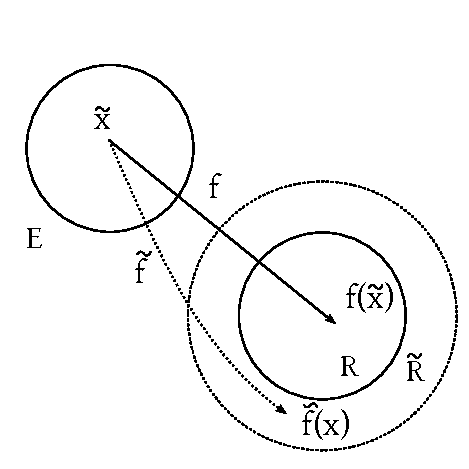
\includegraphics{img/error_map.pdf}
    \caption{Map of the error with $\tilde f$ instead of $f$}
    \label{img:error-map}
  \end{center}
\end{figure}

\index{Stability indicator}
\begin{definition}[Forward stability]
  Let $\tilde f$ be the floating point implementation of an algorithm to solve problem $(f, x)$ of relative normwise condition $\kappa_{\operatorname{rel}}$.
  The \emph{stability indicator} of a normwise forward analysis is the smallest number $\sigma \geq 0$, such that for all $\tilde x \in E$ it holds that
  \[ \frac{\Norm{\tilde f(\tilde x) - f(\tilde x)}}{\Norm{f(\tilde x)}} \leq \sigma \kappa_{\operatorname{rel}} \varepsilon \qquad \text{ for } \varepsilon \to 0 \]
\end{definition}

\subsection{Stability of the componentwise forward analysis}

$\overline{\kappa}_{\operatorname{rel}}$ is the smallest number $\sigma \geq 0$ such that
\[ \max_i \frac{\Abs{\tilde f_i(\tilde x) - f_i(\tilde x)}}{\Abs{f_i(\tilde x)}} \dotted{\leq} \sigma \cdot \overline{\kappa}_{\operatorname{rel}} \varepsilon \qquad \text{ for } \varepsilon \to 0 \]
where $\overline{\kappa}_{\operatorname{rel}}$ is the componentwise relative conditioning of $(f, x)$.
\index{Stable algorithm}
We call algorithm $\tilde f$ \emph{stable} in regards of forward analysis if $\sigma$ is smaller than the number of consecutively executed elementary operations.

\begin{lemma}
  For the elementary operations $\Set{+, -, \cdot, /}$ and the floating point implementations $\Set{\hat{+}, \hat{-}, \hat{\cdot}, \hat{/}}$ it holds that $\sigma \kappa_{\operatorname{rel}} \leq 1$.
\end{lemma}
\begin{proof}
  For every floating point implementation it holds that
  \[ x \hat{*} y = (x * y)(1 + \delta) \qquad * \in \Set{+, -, \cdot, /} \]
  by Lemma~\ref{lemma:2-4} for some $\delta$ with $\Abs{\delta} \leq \varepsilon$.
  Thus,
  \[ \frac{\Abs{x \hat{*} y - x * y}}{x * y} = \frac{\Abs{(x * y)(1 + \delta) - x * y}}{\Abs{x * y}} = \Abs{\delta} \leq 1 \cdot \varepsilon \]
\end{proof}

This approach is rather impractical (determination of the conditioning number of the problem is difficult).

\begin{figure}[!ht]
  \begin{center}
    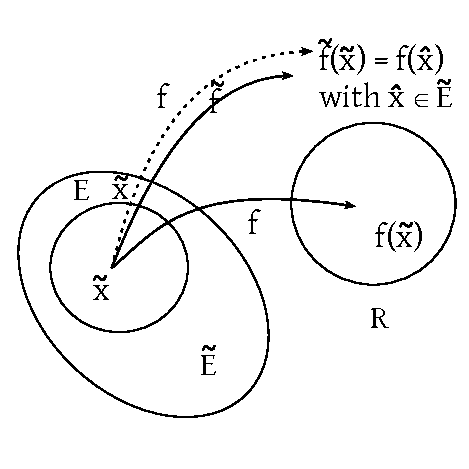
\includegraphics{img/backwards-analysis.pdf}
    \caption{Backwards analysis}
    \label{img:backwards-analysis}
  \end{center}
\end{figure}

\index{Unstable algorithm}
\textbf{Idea:} interpret the error in the algorithm like an input error.
The result $\tilde y = \tilde f(\tilde x)$ is considered as the exact result $\tilde y = f(\hat{x})$ for distorted data $\hat{x}$.
$E = \SetDef{\tilde x}{\Norm{\tilde x - x} \leq \varepsilon \Norm{x}}$.
This is only possible if $\tilde y$ is a admissible solution of $f$ at all.
In the other case, we call the algorithm \emph{unstable}.

\index{Normwise backwards error}
\index{Stability indicator}
\begin{definition}
  The \emph{normwise backwards error} of the algorithm $\tilde f$ to solve the problem $(f, x)$ is the smallest number $\eta \geq 0$,
  for which $\forall \tilde x \in E_\varepsilon$ some $\hat{x}$ exists such that
  \[ \frac{\Norm{\hat{x} - \tilde x}}{\Norm{\tilde x}} \dotted{\leq} \eta \qquad \text{ for } \varepsilon \to 0 \]
  The \emph{componentwise backwards error} is defined as
  \[ \max_i \frac{\Abs{\hat{x}_i - \tilde{x}_i}}{\Abs{\tilde x_i}} \dotted{\leq} \eta \qquad \text{ for } \varepsilon \to 0 \]
  The algorithm is called \emph{stable} (in regards of backwards analysis) with respect to the relative input error $\varepsilon$ if $\eta < \varepsilon \cdot \text{ number of elementary operations}$.
  For given $\varepsilon$ we define a \emph{stability indicator} of the backwards analysis as quotient
  \[ \sigma_R \coloneqq \frac{\eta}{\varepsilon} \]
\end{definition}

\begin{lemma}
  \label{lemma:2-15}
  For stability indicators $\sigma$ and $\sigma_R$, of the forward/backward analysis respectively, it holds that $\sigma \leq \sigma_R$.
  Especially by backwards stability, forwards stability follows.
\end{lemma}
\begin{proof}
  By definition of the backwards error, for every $\tilde x \in E$ there exists some $\hat{x}$ such that $f(\hat{x}) = \tilde f(\tilde x)$ and
  \[ \frac{\Norm{\hat{x} - \tilde x}}{\Norm{\tilde x}} \dotted{\leq} \eta = \sigma_R \cdot \varepsilon \qquad \text{ for } \varepsilon \to 0 \]
  For the relative error in the result, we have
  \[ \frac{\Norm{\tilde f(\tilde x) - f(\tilde x)}}{\Norm{f(\tilde x)}} = \frac{\Norm{f(\hat{x}) - f(\tilde x)}}{\Norm{f(\tilde x)}} \dotted{\leq} \kappa_{\operatorname{rel}} \frac{\Norm{\hat{x} - \tilde{x}}}{\Norm{\tilde{x}}} \dotted{\leq} \kappa_{\operatorname{rel}} \cdot \sigma_R \cdot \varepsilon \qquad \text{ (for $\varepsilon \to 0$)} \]
\end{proof}
\begin{Remark}
  $Ax = b$ with solution $\tilde x$, approximation $\hat{x}$.
  Error $\Norm{\hat{x} - \tilde x}$ is not computable, because $\tilde x$ is unknown.
  Residue $\Norm{b - A\hat{x}}$.
\end{Remark}

\subsection{Backwards analysis for linear equation systems} % 2.4  TODO wrong numbering

\textbf{Question:} Is the LU decomposition a backwardsstable algorithm?

In the following, we will use the following notation for vectors and matrices:
\[ \Abs{A} \leq \Abs{B} \iff \Abs{a_{ij}} \leq \Abs{b_{ij}} \forall i,j \]

\begin{lemma}
  \label{lemma:2-16}
  The floating point implementation of the scalar product
  \[ \IP{x}{y} \coloneqq x_n y_n + \IP{x^{n-1}}{y^{n-1}} \]
  with $x^{n-1} \coloneqq (x_1, \dots, x_{n-1})^T$ and $y^{n-1} \coloneqq (y_1, \dots, y_{n-1})^T$
  denotes some solution $\IP{x}{y}_{\text{rd}} \coloneqq \operatorname{rd}(\IP{x}{y})$ for some $x, y \in \mathbb R^n$
  such that $\IP{x}{y}_{\operatorname{rd}} = \IP{\hat{x}}{y}$ for some $\hat{x} \in \mathbb R^n$ with $\Abs{x - \hat{x}} \dotted{\leq} n \varepsilon \Abs{x}$,
  hence the relative componentwise backwards error is $\eta \leq n \cdot \varepsilon$
  and the scalar product is stable in regards of backwards analysis (with $2n-1$ elementary operations by the scalar product). % TODO too long sentence
\end{lemma}
\begin{proof}
  We need to prove:
  \[ \forall i: \Abs{x_i - \hat{x}_i} \leq \underbrace{n \varepsilon \Abs{x_i}}_{h(\varepsilon)} + \overbrace{\sigma(\Norm{h(\varepsilon)})}^{\sigma} \qquad \text{ for $\varepsilon \to 0$ with } \lim_{\varepsilon \to 0} \frac{\Norm{\varphi(\varepsilon)}}{\Norm{h(\varepsilon)}} = 0 \]
  Thus, we look for a function that converges superlinear towards $0$ for $\varepsilon \to 0$ ($\mathcal O(\varepsilon)$).

  We use induction over $n$ to prove this.
  For $n=1$, the statement is true by Lemma~\ref{lemma:2-4}.
  Now let $n > 1$ and let the statement be true for $n - 1$. For floating point implementation of recursion it is true that
  \[ {\IP xy}_{\operatorname{rd}} = (x_n y_n (1 + \delta) + \IP{x^{n-1}}{y^{n-1}}_{\operatorname{rd}}) (1 + \tilde{\delta}) \]
  where $\Abs{\delta} \leq \varepsilon$ and $\Abs{\tilde \delta} \leq \varepsilon$ characterize the relative error of multiplication and addition respectively.

  By the induction hypothesis, it holds that $\IP{x^{n-1}}{y^{n-1}}_{\operatorname{rd}} = \IP{z}{y^{n-1}}$ for some $z \in \mathbb R^{n - 1}$ with
  \[ \Abs{x^{n-1} - z} \leq (n - 1) \varepsilon \Abs{x^{n-1}} + \mathcal O(\varepsilon) \]
  By $\hat{x}_n = x_n (1 + \delta)(1 + \tilde\delta)$ and $\hat{x}_k = z_k (1 + \tilde\delta)$ by $k = 1, \dots, n-1$ it follows that
  %\[ \Norm{x^{n-1} - z} \leq (n - 1) \varepsilon \Abs{x^{n-1}} \]
  %With $\hat{x_n} = x_n(1 + \delta)(1 + \tilde \delta)$ and $\hat{x}_{\kappa} = z_k(1 + \tilde \delta)$ for $k = 1, \dots, n-1$ it follows that
  \begin{align*}
    {\IP xy}_{\operatorname{rd}} &= x_n y_n(1 + \delta)(1 + \tilde \delta) + \IP{z(1 + \varepsilon)}{y^{n-1}} \\
      &= \hat{x}_n y_n + \IP{\hat{x}^{n-1}}{y^{n-1}} = \IP{\hat{x}}{y} \\
      &\text{ with } \Abs{x_n - \hat{x}_n} \leq 2 \varepsilon \Abs{x_n} + \Abs{x_n} \Abs{y_n} \delta \tilde \delta \\
      &\leq n \varepsilon \Abs{x_n} + \mathcal O(\varepsilon) \\
    \text{ and } \Abs{x_k - \hat x_k} &\leq \Abs{x_k - z_k} + \Abs{x_k - \hat{x}_k} \\
      &\leq (n - 1) \varepsilon \Abs{x_k} + \mathcal O(\varepsilon) + \varepsilon \Abs{z_k} \\
      &\leq n \varepsilon \Abs{x_k} + \mathcal O(\varepsilon) \text{ for } k = 1, \dots, n-1
  \end{align*}
  The last estimate can be made using
  \[ \Abs{z_k} - \Abs{x_k} \leq \Abs{x_k - z_k} \leq (n - 1) \varepsilon \Abs{x_k} + \mathcal O(\varepsilon) \]
  \[ \implies \varepsilon \Abs{z_k} \leq \varepsilon \Abs{x_k} + \mathcal O(\varepsilon) \]
\end{proof}

\begin{theorem}
  \label{theorem:2-17}
  The floating point implementation of forward substitution to solve a linear equation system $Lx = b$ with some lower triangular matrix $L$ computes the solution $\hat{x}$ such that there exists some lower triangular matrix $\hat L$ with $\hat L \hat x = b$ and $\Abs{L - \hat L} \dotted{\leq} n \varepsilon \Abs{L}$.
  Hence for componentwise relative backwards errors, we have $\eta \leq n \cdot \varepsilon$ and the forward substitution is stable in regards of backwards analysis.
\end{theorem}
\begin{proof}
  Again, we will use a recursive approach.
  \[ l_{kk} x_k = b_k - \IP{l^{k-1}}{x^{k-1}} \]
  For $k = 1, \dots, n$, we have
  \begin{align*}
    x^{k-1} &\coloneqq (x_1, \dots, x_{k-1})^T \text{ and } \\
    l^{k-1} &\coloneqq (l_{k,1}, \dots, l_{k,k-1})^T
  \end{align*}
  In floating point arithmetics, the following recursion is yielded,
  \[ l_{kk}(1 + \delta_k)(1 + \tilde \delta_k) \hat{x}_k = b_k - \IP{l^{k-1}}{x^{k-1}}_{\operatorname{rd}} (1 + \tilde \delta_k) \]
  where $\delta_k, \tilde \delta_k$ with $\Abs{\delta_k} \leq \varepsilon$ and $\Abs{\tilde\delta_k} \leq \varepsilon$ are the relative errors of multiplication/addition.
  By Lemma~\ref{lemma:2-16}, it follows that
  \[ \IP{l^{k-1}}{\hat{x}^{k-1}}_{\operatorname{rd}} = \IP{\tilde l^{k-1}}{\hat{x}^{k-1}} \]
  for some vector $\tilde l^{\tilde k - 1} = (\tilde l_{k,1}, \dots, \tilde l_{k,k-1})^T$
  with $\Abs{l^{k-1} - \tilde l^{k-1}} \dotted{\leq} (k - 1) \varepsilon \Abs{l^{k-1}}$.
  Now let $\hat{l}_{kk} \coloneqq l_{kk} (1 + \delta_k)(1 + \tilde \delta_k)$ and $\hat{l}^{k-1} \coloneqq (1 + \tilde \delta_k) \tilde l^{k-1}$ then
  \begin{align*}
    \Abs{\hat{l}^{k-1} - l^{k-1}} &\dotted{\leq} (k-1) \varepsilon \Abs{l^{k-1}} + \Abs{\tilde \delta_k} \Abs{\tilde l^{k-1}} \\
      &\dotted{\leq} k \varepsilon \Abs{l^{k-1}} \\
    \Abs{\hat{l}_{kh} - l_{kj}} &\dotted{\leq} 2 \varepsilon
  \end{align*}
  \[ \implies \hat{L} \hat{x} = b \land \Abs{L - \hat{L}} \dotted{\leq} n \varepsilon \Abs{L} \]
\end{proof}

\dateref{2018/10/18}

\begin{lemma}
  \label{lemma:2-18}
  Let $A$ have a LU decomposition. Then Gaussian elimination determines $\hat L$ and $\hat U$ such that $\hat L \hat U = \hat A$ for some matrix $\hat A$ with
  \[ \Abs{A - \hat A} \dotted{\leq} n \Abs{\hat L} \Abs{\hat U} \varepsilon \]
\end{lemma}

\begin{theorem}
  \label{theorem:2-19}
  $A$ has some LU-decomposition. 
  Then Gaussian elimination for linear equation system $Ax = b$ gives a solution $\hat x$ with $\hat A \hat x = b$ for some matrix $\hat A$ with
  \[ \Abs{A - \hat A} \dotted{\leq} 2n \Abs{\hat L} \Abs{\hat U} \varepsilon \]
\end{theorem}

\begin{theorem}
  \label{theorem:2-20}
  The Gaussian elimination with column pivot strategy for the linear equation system $Ax = b$ determines some $\hat x$ such that $\hat A \hat x = b$ for some matrix $\hat A$ with
  \[ \frac{\Norm{A - \hat A}_{\infty}}{\Norm{A}_\infty} \dotted{\leq} 2n^3 \rho_n(A) \varepsilon \qquad \text{ where } \rho_n(A) \coloneqq \frac{\alpha_{\operatorname{max}}}{\max_{i,j} \Abs{a_{ij}}} \]
  and where $\alpha_{\operatorname{max}}$ is the largest absolute value of an element that occurs during elimination in the remainder matrices $A^{(1)} = A$ to $A^{(n)} = U$.
\end{theorem}

\[ A = \begin{bmatrix} 1 & 0 & \dots & 0 & 1 \\ -1 & \vdots & \ddots & \vdots & \vdots \\ \vdots & \ddots & \ddots & & \\ -1 & \dots & \dots & -1 & 1 \end{bmatrix} \]
For matrix $A$ it holds that $\rho_n(A) = 2^{n-1}$.

Consider that the previous result also provides \emph{no} positive statement about the backwards stability of the LU decomposition.

\section{Linear least squares}

\textbf{Goal:} Solution of overdetermined linear equation systems
\[ Ax = b \qquad A \in \mathbb R^{m \times n} \qquad m > n \qquad b \in \mathbb R^m \]
by the method of linear least squares.

For this, we are going to use (numerically stable) orthogonal transformations.

\subsection{Gaussian process of least squares}

\textbf{Problem:} Given $m$ input data points ($t_i, b_i$) and $t_i, b_i \in \mathbb R$ for $i = 1, \dots, m$.
They describe the values $b_i$ of an object at timestamp $t_i$.

\index{Modelling function}
We assume that there exists an underlying law such that the dependency of $b$ and $t$ can be represented by some \emph{modelling function} $\varphi$ with $b(t) = \varphi(t_i; x_1, \dots, x_n)$. The modelling function therefore takes $n$ unknowns $p_i$.

\begin{example}[Ohm's law]
  Consider Ohm's law $b = xt = \varphi(t_i x)$ where $t$ denotes the current, $b$ the voltage and $x$ resistance.
\end{example}

So want to approximate data points in the $\mathbb R^2$ plane linearly.

If the model would be \emph{exact} and if you have no errors in measurement, then we are supposed to evaluate parameters $x_1, \dots, x_n$ such that $b_i = b(t_i) = \varphi(t_i; x_1, \dots, x_n)$ for $i = 1, \dots, m$.

In reality, measurements are subject to errors and modelling functions are also just approximations of reality.
We therefore require that $b_i \approx \varphi(t_i; x_1, \dots, x_n)$ for $i = 1, \dots, m$.
We weight the individual deviations
\[ \Delta i \coloneqq b_i - \varphi(t_i; x_1, \dots, x_n) \qquad i = 1, \dots, m \]
By Gauss, determine $x_i$ such that $\sum_{i=1}^m \Delta i^2$ becomes minimal.
We use the short notation $\Delta^2 \coloneqq \sum_{i=1}^m \delta_i^2 \implies \operatorname{min}$.
Often it is more useful to weight the individual deviations differently.
For some measurement precision $\delta b$, introduce weights
\[ \sum_{i=1}^m \left(\frac{\Delta i}{\delta b_i}\right) \to \text{ min} \]
We consider the special case of linear (with respect to $x$) modelling functions $\varphi$, hence $\varphi(t_i; x_1, \dots, x_n) = a_1(t) x_1 + \dots + a_n(t) x_n$ where $a_1, \dots, a_n: \mathbb R \to \mathbb R$ are arbitrary functions.
Furthermore we choose $\Norm{} = \Norm{}_2$.
We can denote the least square problem as
\[ \Norm{b - Ax} \to \operatorname{min} \qquad \text{ where } b = \begin{pmatrix} b_1 \\ \vdots \\ b_m \end{pmatrix}, x = \begin{pmatrix} x_1 \\ \vdots \\ x_n \end{pmatrix} \]
\[ \text{and } A = (a_{ij}) \in \mathbb R^{m \times n} \text{ with } a_{ij} \coloneqq a_j(t_i) \]

\subsection*{Orthogonal equations}

We look for some point $z = Ax$ of the image space $U(A)$ of $A$, that has the smallest distance to some given $b$.
$Ax$ is the orthogonal projection of $b$ to the subspace $U(A) = \operatorname{image}(A)$.

\begin{theorem}
  \label{theorem:3-2}
  Let $V$ be a vector space of $\dim{V} < \infty$ with scalar product $\IP{}{}$.
  Let $U \subset V$ be a subspace. Let
  \[ U^\bot = \SetDef{v \in V}{\IP{v}{u} = 0 \forall u \in U} \]
  be the orthogonal complement in $V$. Then for all $v \in V$ with respect to the norm induced by $\Norm{v} = \sqrt{\IP vv}$ such that
  \[ \Norm{v - u} = \min_{\tilde u \in U} \Norm{v - \tilde u} \iff v - u \in U^\bot \]
\end{theorem}

Proof sketch:
\begin{itemize}
  \item $V = U \oplus U^\bot$
  \item $v = u + w, u \in U, w \in U^\bot$ unique
  \item $\tilde u \in U$ arbitrary:
    \[ \Norm{v - \tilde u}^2 = \Norm{(v - u) + (u - \tilde u)}^2 = \Norm{v - u}^2 + \Norm{u - \tilde u}^2 \geq \Norm{v - u}^2 \]
    with $v - u = w$ and $(u - \tilde u) \in U$.
\end{itemize}

\dateref{2018/10/23}

\index{Orthogonal projection}
The unique solution $u \in U$ of $\min{\Norm{v - u}}$ is called \emph{orthogonal projection} of $V$ to $U$.
The map $P: V \to U$ with $v \mapsto Pv$ with $Pv = u$ is linear and is called \emph{orthogonal projection} of $V$ to $U$.

\begin{remark}
  \label{rem-3-3}
  We get an analogous statement if we replace $U$ by an affine subspace $W = w_0 + U \subseteq V$ where $w_0 \in V$.
  $U$ is the parallel, to $W$, linear subspace of $V$.

  For all $v \in V$, $w \in W$: $\Norm{v - w} = \min_{\tilde w \in w} \Norm{v - \tilde w} \iff v-w \in U^\bot$.
\end{remark}

\index{Orthogonal equations}
\begin{theorem}
  \label{theorem:3-4}
  The vector $x \in \mathbb R^n$ is a solution of the linear least squares problems $\min{\Norm{b - Ax}} \iff x$ satisfies the so-called orthogonal equations $A^T Ax = A^T b$~\dt{Normalengleichungen}.

  Especially, the linear least squares problem is uniquely solvable iff $A$ has full column rank.
\end{theorem}

\begin{proof}
  By Theorem~\ref{theorem:3-2}, $V \coloneqq \mathbb R^n$, $U \coloneqq \operatorname{image}(A) = \operatorname{rank}(A)$.
  \begin{align*}
    \implies \max{\Norm{b - Ax}} &\iff \IP{b - Ax}{A \tilde x} = 0 \forall \tilde x \in \mathbb R^n \\
      &\iff 0 = \IP{A^t (b - Ax)}{\tilde x} \forall \tilde x \in \mathbb R^n \\
      &\iff A^t (b - Ax) = 0 \\
      &\iff A^t b = A^t Ax
  \end{align*}
  Thus the first statement is proven. How about the second statement?
  \begin{align*}
    A^t A \text{ regular } &\iff \operatorname{rank}(A) = n
  \end{align*}
\end{proof}

\begin{Remark}[Geometric interpretation]
  $b - Ax$ is orthogonal to $\operatorname{range}(A)$ with $A \subseteq \mathbb R^n$.
\end{Remark}

\textbf{Solution of the orthogonal equation system:}
Theoretically, we can create $A^T A$ and retrieve a symmetric positive definite matrix ($\implies$ decomposition with Cholesky process).

\begin{Remark}[Computing time]
  \begin{enumerate}
    \item Determination of $A^t A$ (only one half, because of symmetry)
      \[ (A^t A)_{ij} = (\IP{a_j}{a_j})_{i,j} \qquad a_j = j\text{-th column of } A \to \frac12 n^2 n \]
    \item Cholesky decomposition $\sim \frac16 n^3$
  \end{enumerate}
  In case of $m \gg n$, the first approach will take over $\implies \sim \frac12 n^2 n$. $\frac23 m^3$ for $n \approx m$.
\end{Remark}

\begin{lemma}
  \label{lemma:3-5}
  For some matrix $A \in \mathbb R^{m \times n}$ with $m \geq n$ and full column rank ($\operatorname{rank}(A) = n$),
  $\kappa_2(A^t A) = (\kappa_2(A))^2$.
\end{lemma}

\begin{proof}
  By definition of condition numbers:
  \begin{align*}
    (\kappa_2(A))^2 &= \frac{\max_{\Norm{x}=1} \Norm{Ax}_2^2}{\min_{\Norm{x} = 1} \Norm{Ax}_2^2} \\
      &= \frac{\max_{\Norm{x}=1} \IP{Ax}{Ax}}{\min_{\Norm{x} = 1} \IP{Ax}{Ax}} \\
      &= \frac{\max \IP{A^t Ax}{x}}{\min \IP{A^t Ax}{x}} & \text{\enquote{Rayleigh eigenvalue}} \\
      &\overset{A^tA \text{sym.}}{=} \frac{\lambda_{\operatorname{max}} (A^t A)}{\lambda_{\operatorname{min}} (A^t A)} \\
      &\overset{A^tA \text{sym.}}{=} \kappa_2(A^t A)
  \end{align*}
\end{proof}

Recognize that the amplification of the error for the orthogonal equation is larger.
Therefore it makes sense to avoid computing $A^T A$ and use the original matrices $A$ and $A^T$ instead, e.g.
\[ \begin{pmatrix} I & A \\ A^T & 0 \end{pmatrix} \begin{pmatrix} r \\ 0 \end{pmatrix} = \begin{pmatrix} b \\ 0 \end{pmatrix} \]
\[ \implies A^T r = 0 \land r \neq Ax = b \]
\[ \implies r = b - Ax \qquad \implies 0 = A^T r = A^T (b - Ax) \]

\[ \Norm{A_3}_2^2 = \max_{\Norm{x}_2 = 1} \Norm{Q_j x}_2^2 = \max_{\Norm{x}_2 = 1} \IP{x}{Q^TQx} = 1 \]
Recognize that $Q^TQ = I$.

\subsection{Orthogonalization process}

We can represent the eliminination process for linear equation systems  (e.g. Gaussian elimination) formally as
\[ A \xrightarrow{f_1} B_1 A \xrightarrow{f_2} B_2 B_1 A \xrightarrow{f_3} \dots \xrightarrow{f_k} B_k \dots B_1 A \dots \rightarrow U \]
where
\[ U = \begin{pmatrix} 1 & * \\ 0 & \varepsilon \end{pmatrix} \]
and where matrices $B_j$ describe the operations applied to matrix $A$.
Through this process, the condition numbers of the individual matrices can be amplified, such that instabilities can occur.
If we instead use orthogonal transformations $Q_j$ for elimination, we have
\[ \kappa_2(Q_j) = \Norm{Q_j}_2 \cdot \Norm{Q_j}^{-1}_2 = \Norm{Q_j}_2 \Norm{Q_j}_2 = 1 \]

Orthogonalization process are necessarily stable, but have higher computing times compared to Gaussian elimination.
If we assume we transformed a given matrix $A \in \mathbb R^{m \times n}$ with $m \geq n$ with some orthogonal matrix $Q \in \mathbb R^{m \times m}$ into upper triangular matrix, then
\[
  Q^T A = \begin{bmatrix}
    *      & \dots   & x \\
           & \ddots  & \vdots \\
           &         & x \\
    0      &         & * \\
    \vdots &         & \vdots \\
    0      &         & 0
  \end{bmatrix} = \begin{bmatrix} U \\ 0 \end{bmatrix}
\]

\begin{theorem}
  \label{theorem:3-6}
  Let $A \in \mathbb R^{m \times n}$, $m \geq n$, of maximum rank $n, b \in \mathbb R^m$ and $Q \in \mathbb R^{m \times m}$ be an orthogonal matrix with
  \[ Q^T A = \begin{bmatrix} U \\ 0 \end{bmatrix} \text{ and } Q^T b = \begin{bmatrix} b_1 \\ b_2 \end{bmatrix} \]
  where $b_1 \in \mathbb R^n$, $b_2 \in \mathbb R^{m - n}$ and $U \in \mathbb R^{n \times n}$ is an (invertible) upper triangular matrix.
  Then $x = U^{-1} b_1$ is the solution of the linear least squares problems $\min\Norm{b - Ax}_2$.
\end{theorem}

\begin{proof}
  Because $Q$ is orthogonal, $\forall x \in \mathbb R^n$ it follows that
  \[ \Norm{b - Ax}_2^2 = \Norm{Q^T (b - Ax)}_2^2 = \Norm{\begin{pmatrix} b_1 - Ux \\ b_2 \end{pmatrix}}_2^2 = \Norm{b_1 - Ux}_2^2 + \Norm{b_2}_2^2 \geq \Norm{b_2}_2^2 \]
  Because $\rank(A) = \rank(U) = n$, $U$ is invertible. The term $\Norm{b_1 - Ux}_2^2$ disappear for $x = U^{-1} b_1$
\end{proof}

\begin{Remark}
  $A$: $0 \neq \Norm{r} = \Norm{b - Ax} = \Norm{b_2}$.
\end{Remark}

What do orthogonal transformations look like?
In general, these transformations are rotations and reflections.

e.g. $x \mapsto \alpha e_1 = Qx$ with $Q = \begin{bmatrix} \cos(\theta) & \sin(\theta) \\ -\sin(\theta) & \cos(\theta) \end{bmatrix}$.

Alternatively, $x \mapsto \alpha e_1 = x = 2\frac{\IP vx}{\IP vv} v$ where $v$ is collinear to the difference $x = \alpha e_1$.

\subsection*{Givens rotations}

\index{Givens rotations}
Givens rotations are described by matrices of form
\[
  Q_{k,l} \coloneqq \begin{bmatrix}
    I &    &   &   & \\
      & c  &   & s & \\
      &    & I &   & \\
      & -s &   & c & \\
      &    &   &   & I
  \end{bmatrix}
  \in \mathbb R^{m \times m}
\]
with proper dimension of the unit matrix and $c^2 + s^2 = 1$. For $x \in \mathbb R^m$ it holds that
\[
  x \mapsto y = Q_{k,l} x \text{ with } y_i = (Q_{k,l} x)_i =
  \begin{cases}
    c x_k + sx_l & i = k \\
    -s x_k + cx_l & i = l \\
    x_i & \text{else}
  \end{cases}
\]
Thus for $A = [a_1, \dots, a_n] \in \mathbb R^{m \times n}$, we get
\[ Q_{k,l} A = [Q_{k,l} a_1, \dots, Q_{k,l} a_n] \]
Hence, only rows $k$ and $l$ of matrix $A$ will be modified.

\textbf{Question:} How to choose $c$ and $s$ to eliminate a component $x_l$ of $x$?
Because $Q_{k,l}$ operates on the $(k,l)$-layer, we consider without loss of generality $m=2$.
By $x_k^2 + x_l^2 \neq 0$ and $s^2 + c^2 = 1$ it follows that
\[ \begin{bmatrix} c & s \\ -s & c \end{bmatrix} \begin{bmatrix} x_k \\ x_l \end{bmatrix} = \begin{bmatrix} r \\ 0 \end{bmatrix} \]
\[ \iff r = \pm \sqrt{x_k^2 + x_l^2}, c = \frac{x_k}{r}, s = \frac{x_l}{r} \]
Computing $x_k^2$ might gives us an exponent overflow.
\[ \tau \coloneqq \frac{x_k}{x_l}, s \coloneqq \frac{1}{\sqrt{1 + \tau^2}}, c \coloneqq s\tau \text{ if } \Abs{x_l} > \Abs{x_k} \]
and accordingly,
\[ \tau \coloneqq \frac{x_l}{x_k}, c = \frac{1}{\sqrt{1 + \tau^2}}, s \coloneqq c\tau \text{ if } \Abs{x_k} \geq \Abs{x_l} \]
Now transform $A$ iteratively into triangular form.

For example, consider
\[ A = \begin{bmatrix} A & * & * & * \\ * & * & * & * \\ * & * & * & * \\ * & * & * & * \\ * & * & * & * \end{bmatrix} \xrightarrow{(5,4)} \begin{bmatrix} * & * & * & * \\ * & * & * & * \\ * & * & * & * \\ * & * & * & * \\ 0 & * & * & * \end{bmatrix} \xrightarrow{(4,3)} \dots \]
\[ \xrightarrow{(2,1)} \begin{bmatrix} * & * & * & * \\ 0 & * & * & * \\ 0 & * & * & * \\ 0 & * & * & * \\ 0 & * & * & * \end{bmatrix} \xrightarrow{(5,4)} \dots \xrightarrow{(4,3)} \dots \xrightarrow{(5,4)} \begin{bmatrix}  * & * & * & * \\ 0 & * & * & * \\ 0 & 0 & * & * \\ 0 & 0 & 0 & * \\ 0 & 0 & 0 & 0 \end{bmatrix} \]
\begin{Remark}[Computing time]
  Computing time for a dense matrix $A \in \mathbb R^{m \times n}$:
  \begin{enumerate}
    \item $\sim \frac{n^2}{2}$ square roots and $\frac43 n^3$ multiplications, if $m \approx n$.
    \item $m \cdot n$ are square root and $2mn^2$ multiplications if $m \ggg n$.
  \end{enumerate}
\end{Remark}
This is an alternative for Gaussian elimination. The algorithm is \emph{more stable}, but \emph{more expensive}.

But it can be advantageous for special matrix, e.g. Hessenberg matrices, which are \enquote{almost triangular} (so the first subdiagonal also contains non-zero entries).
Here, we need $n-1$ Givens rotations if we want to achieve upper triangular form.

\subsection*{Householder reflections}
\dateref{2018/10/25}

\index{Householder reflections}
For given $0 \neq v \in \mathbb R^m$, we define the matrix $Q \in \mathbb R^{m \times m}$.
\[ Q = I - 2 \frac{vv^T}{v^Tv} \]

They describe reflections on the mirror plane, which are vertical to $v$.
The following properties hold:
\begin{enumerate}
  \item symmetry: $Q = Q^T$
  \item orthogonality: $QQ^T = I$
  \item $Q^2 = \operatorname{id}$, thus $Q$ is \emph{involutional}
  \item $\operatorname{spec}(Q) = \Set{\pm 1}, -1$ simple, $1$ $(n-1)$-times.
\end{enumerate}

For $y \in \mathbb R^n$,
\[ y \mapsto Qy = \left(I - 2 \frac{vv^T}{v^T v}\right) y = y - 2 \cdot \frac{\IP vy}{\IP vv} \]

\textbf{Question}: How can we achieve that $Q$ maps vector $y$ to $\alpha \cdot e_1$? Hence,
\[ \alpha \cdot e_1 = y - 2 \frac{\IP vy}{\IP vv} \cdot v \in \operatorname{span}(e_1) = \alpha(\Set{e_1}) \]

Consider that
\[ \Abs{\alpha} = \Norm{\alpha e_1} = \Norm{y - 2 \frac{\IP vy}{\IP vv} v}_2 = \Norm{Qy}_2 = \Norm{y}_2 \]
and $y \in \operatorname{span}(y - \alpha \cdot e_1)$.
This way we can retrieve $Q$ by,
\[ v \coloneqq y - \alpha e_1 \qquad \alpha = I \Norm{y}_2 \]
To avoid elimination (or subtraction) in $v = (y_1 - \alpha, y_2, \dots, y_n)^T$, choose $\alpha \coloneqq -\operatorname{sign}(y_1) \cdot \Norm{y}_2$. Now,
\[ \IP vv = \IP{y - \alpha e_1}{y - \alpha e_1} = \Norm{y}^2 - 2\alpha \IP{e_1}{y} + \alpha^2 = 2\alpha^2 - 2\alpha \IP{e_1}{y} = -2\alpha (y_1 - \alpha) \]
$Qy$ for $y \in \mathbb R^m$ can be determined by
\[ Qy = y - 2 \frac{\IP vy}{2(y_1 - \alpha)} \cdot v \]
In a first step choose $Q_1$ (where $A \in \mathbb R^{m \times n}$):
\[ [a_1 \dots a_n] = A \to A' = Q_1 \cdot A = \begin{bmatrix} \alpha_1 & \\ 0 & \\ \vdots & a_2' \dots a_n' \\ 0 & \end{bmatrix} \]
where $Q_1 = I - 2 \frac{v_1 v_1^T}{v_1^T v_1}$ with $v_1 \coloneqq a_1 - \alpha_1 e_1$ and $\alpha_1 \coloneqq -\operatorname{sign}(a_{11}) \cdot \Norm{a_1}$.

After the $k$-th step, we get
\[ A^{(k)} = \begin{bmatrix} * & & & * \\ & \ddots & & \\ & & * & \\ 0 & & & T^{(k+1)} \end{bmatrix} \]
with $T^{(k+1)} \in \mathbb R^{m-k \times n-k}$. Now we create orthogonal matrix
\[ Q_{k+1} \coloneqq \begin{bmatrix} I & 0 \\ 0 & \tilde Q_{k+1} \end{bmatrix} \]
where $\tilde Q_{k+1}$ modifies matrix $T^{(k+1)}$. The next subcolumn will be eliminated.

After $p = \min(m,n)$ steps, we retrieve an upper triangular matrix
\[ R = Q_p \dots Q_1 \cdot A \]
\[ \iff A = QR \text{ where } Q = Q_1 \cdot \dots \cdot Q_p \]

% TODO static reference
Based on Theorem~2.6, we retrieve the following process:
\begin{enumerate}
  \item $A = QR$ ($QR$ decomposition using Householder or Givens)
  \item $\begin{pmatrix} b_1 \\ b_2 \end{pmatrix} = Q^t b$ with $b_1 \in \mathbb R^n$ and $b_2 \in \mathbb R^{m-n}$ (transformation of $b$)
  \item $Rx = b_1$ (solving by backwards substitution)
\end{enumerate}

\begin{Remark}[Implementation]
  Usually, we store the Householder vectors $v_1, \dots, v_p$ in the lower half of $A$ and the diagonal elements $v_{1i} = \alpha_i$ with $i = 1,\dots,p$ in a separate vector.
\end{Remark}

\begin{Remark}[Computing time]\hfill{}
  \begin{itemize}
    \item $\sim 2n^2m$ multiplications if $m \gg n$
    \item $\frac23 n^3$ if $m \approx n$
  \end{itemize}
\end{Remark}

It is important to recognize that this process is numerically stable!

\subsection{Singular value decomposition} % TODO chapter 3.3

Literature:
\begin{itemize}
  \item Gene H. Golub and Charles F. Van Loan: \enquote{Matrix computations}
\end{itemize}

If $A \in \mathbb R^{m \times n}$ has non-full rank $n$,
then the linear equation system of $\min \Norm{b - Ax}$ is not unique,
because $\forall \tilde x: \Norm{b - A\tilde x} = \Norm{b - A(\tilde x + v)} \forall v \in \ker(A)$.

Are there more decompositions of the matrix?

Recognize that the QR decomposition always exists anyways.

\begin{theorem}
  \label{theorem:3-7}
  Let $A \in \mathbb R^{m \times n}$.
  There $\exists U \in \mathbb R^{m \times m}, V \in \mathbb R^{n \times n}:
  U^T U = I, V^T V = I$ and $A = U \Sigma V^T$ with $\Sigma \in \mathbb R^{n \times n}$
  where $\Sigma = \operatorname{diag}(\sigma_1, \dots, \sigma_p), p = \min(m, n), V = [v_1, \dots, v_n]$
  and $\sigma_1 \geq \sigma_2 \geq \dots \geq \sigma_p \geq 0$.
\end{theorem}

\index{Singular values of a matrix}
\index{Singular vectors of a matrix}
\begin{remark}
  $\sigma_i$ are called \enquote{singular values} of $A$.
  $u_i$ and $v_i$ are called left- and right-singular vectors of $A$.
\end{remark}

\dateref{2018/10/30}

\begin{proof}
  Let $x \in \mathbb R^n$ and $y \in \mathbb R^m$ such that $\Norm{x}_2 = 1 = \Norm{y}_2$ and $Ax = \sigma y$ where $\sigma = \Norm{A}_2$.
  Recognize that $x,y$ exist because $\Norm{A}_2 = \sup_{\Norm{\tilde x} = 1} \Norm{A\tilde x}_2 = \max_{\Norm{\tilde x}_2 = 1} \Norm{A\tilde x}_2$.

  Hence, there exists $x$ with $\Norm{x}_2 = 1$ and $\Norm{Ax}_2 = \Norm{A}_2$.
  Followingly, we define $y \coloneqq \frac{Ax}{\Norm{A}_2}$ and it is true that $\sigma y = Ax$.
  \[ \Norm{y}_2 = \frac{\Norm{Ax}_2}{\Norm{A}_2} = 1 \]
  We construct orthonormal bases $\Set{x, v_2, \dots, v_n}$ and $\Set{y, u_2, \dots, u_m}$.
  The corresponding matrices $U = \begin{bmatrix} y & u_2 & \dots & u_m \end{bmatrix}$ and $V = \begin{bmatrix} x & v_2 & \dots & v_n \end{bmatrix}$ are orthogonal. $V^T V = I$, $U^T U = I$. Let $U_2 \coloneqq (u_2, \dots, u_m)$ and $V_2 \coloneqq (v_2, \dots, v_n)$. Furthermore,
  \[
    U^T AV
      = \begin{bmatrix} y^T \\ U_2^T \end{bmatrix} A \begin{bmatrix} X & V_2 \end{bmatrix}
      = \begin{bmatrix} y^T Ax & y^T A V_2 \\ U_2^T Ax & U_2^T AV_2 \end{bmatrix}
      = \begin{bmatrix} \sigma & w^T \\ 0 & B \end{bmatrix} \coloneqq A_1
  \]
  where $w \in \mathbb R^{n - 1}$ and $B \in \mathbb R^{m - 1 \times n-1}$ because
  $\Norm{A_1 \left(\begin{bmatrix} \sigma \\ w \end{bmatrix}\right)}_2^2 \geq (\sigma^2 + w^T w)$
  it holds that $\Norm{A_1}_2^2 \geq (\sigma^2 + w^T W)$.
  On the other hand, $\sigma^2 = \Norm{A}_2^2 = \Norm{A_1}_2^2$. Thus $w = 0$.
  The statement then follows inductively.
\end{proof}

\subsection*{Properties of the singular value decomposition}

\begin{corollary}
  \label{cor-3-9}
  If $A = U \Sigma V^T \in \mathbb R^{m \times n}$ and $m \geq n$ is the singular value decomposition of $A$,
  then $Av_i = \sigma_i u_i$ and $A^T u_i = \delta_i v_i$ for all $i = 1, \dots, n$.
\end{corollary}

\begin{proof}
  Consider columnwise the equality $AV = U \Sigma$ and accordingly, $A^T U = V\Sigma^T$.
\end{proof}

By the corollary, it immediately follows that
\[ A^T A v_i = \sigma_i^2 v_i \qquad A A^T u_i = \sigma_i^2 u_i \]
hence the squares of singular values are the eigenvalues of the matrices $A^T A$, and accordingly $A A^T$.

\textbf{Illustrative interpretation:}
The singular values of a matrix $A$ give the length of the semi-axes of the ellipsis defined by $E = \SetDef{Ax}{\Norm{x}_2 = 1}$.
The directions of semi-axes are denotes by $u_i$.

\[ \Norm{A}_2^2 = \sup_{x \neq 0} \frac{\IP{Ax}{Ax}}{\IP{x}{x}} = \sup_{x \neq 0} \frac{\IP{A^TAx}{x}}{\IP xx} = \lambda_{\max}(A^T A) \]

\begin{corollary}
  \label{corollary-3-10}
  Let $A \in \mathbb R^{m \times n}$. Then,
  \[ \Norm{A}_2 = \sigma_1 \qquad \Norm{A}_F = \sqrt{\operatorname{trace}(A^T A)} = \sqrt{\sigma_1^2 + \dots + \sigma_p^2} \]
\end{corollary}

\begin{proof}
  Consider that for spectral norm and Frobenius norm, it holds that $\Norm{A} = \Norm{U^T A V} = \Norm{\Sigma}$.
\end{proof}

\begin{corollary}
  \label{cor-3-11}
  If $A$ has exactly $r$ positive singular values,
  then $r K(A) =  r$ and $\ker(A) = \operatorname{span}\Set{v_{r+1}, \dots, v_n}$ and $\operatorname{range}(A) = \operatorname{span}\Set{u_1, \dots, u_r}$.
\end{corollary}

\begin{proof}
  Because $U$ and $V$ are regular, it holds that $\rank(A) = \rank(U \Sigma V^T) = \rank(\Sigma) = r$.

  The statements regarding the kernel and image of $A$ result by Corollary~\ref{cor-3-9}.
\end{proof}

\begin{corollary}
  \label{cor-3-12}
  Let $A \in \mathbb R^{m \times n}$ and $\rank(A) = r$. Then $A = \sum_{i=1}^r \sigma_i u_i v_i^T$.
\end{corollary}

\begin{proof}
  Again, consider the matrix notation of the singular value decomposition:
  \[
    A = (U \Sigma) V^T
    = \begin{bmatrix} \sigma_1 u_1 & \sigma_2 u_2 & \dots & \sigma_r u_r & 0 & \dots & 0 \end{bmatrix} \begin{bmatrix} v_1^T \\ \vdots \\ v_n^T \end{bmatrix}
    = \sum_{r=1}^r \sigma_i u_i v_i^T
  \]
\end{proof}

\begin{theorem}[Eckart-Young-Mirsky]
  \label{theorem:3-13}
  If $k < r = \rank(A)$ and $A_k = \sum_{i=1}^k \sigma_i u_i v_i^T$,
  then $\min_{\rank(B) = k} \Norm{A - B}_2 = \Norm{A - A_k}_2 = \sigma_{k+1}$.
\end{theorem}

\begin{proof}
  Because $U^T A_k V = \diag(\sigma_1, \dots, \sigma_k, 0, \dots, 0)$, $\rank(A_k) = k$. Furthermore,
  \[ \Norm{U^T (A - A_k) V}_2 = \diag(0, \dots, 0, \sigma_{k+1}, \dots, \sigma_p) \]
  and therefore $\Norm{A - A_k}_2 = \sigma_{k+1}$.
  Now let $B \in \mathbb R^{m \times n}$ with $\rank(B) = k$ arbitrary.
  Then we can find an orthonormal basis $x_1, \dots, x_{n-k}$ such that $\ke(B) = \operatorname{span}\Set{x_1, \dots, x_{n - k}}$.
  Furthermore it holds that $\operatorname{span}\Set{x_1, \dots, x_{n-k}} \cap \operatorname{span}\Set{v_1, \dots, v_{k+1}} \neq \Set{0}$.
  Let $z$ with $\Norm{z}_2 = 1$ of this intersection.
  Then $Bz = 0$ and $Az = A \sum_{i=1}^{k+1} \alpha_i v_i = \sum_{i=1}^{k+1} \sigma_i \alpha_i u_i$.
  Because $\Norm{z}_2 = 1$, $1 = \Norm{z}_2^2 = \Norm{\sum_{i=1}^{k+1} \alpha_i v_i}_2^2 = \sum_{i=1}^{k+1} \alpha_i^2$.
  Followingly,
  \[ \Norm{A - B}_2^2 \geq \Norm{(A - B) z}_2^2 = \Norm{Az}_2^2 = \sum_{i=1}^{k+1} \sigma_i^2 \alpha_i^2 \geq \sigma_{k+1}^2 \underbrace{\sum_{i=1}^{k+1} \alpha_i^2}_{= 1} = \sigma_{k+1}^2 \]
\end{proof}

We go back to the topic of $\min_x \Norm{b - Ax}_2$.

Consider the equation $b \cdot Ax = d$ and we followingly want to minimize the norm of the residue $\Norm{d}_2$.
Left-sided multiplication with $U^T$ gives
\[ U^T (b - Ax) = U^T d \implies U^T b - U^T AVV^T x = U^T d = \tilde d \]
Because of orthogonality of $U$, $\Norm{\tilde d}_2 = \Norm{d}_2$ and thus we can minimize $\Norm{\tilde d}_2$.
For this we introduce auxiliary vectors $\tilde x = V^T x \in \mathbb R^n$ and $\tilde b = U^T b \in \mathbb R^m$.
Because of the singular value decomposition, we retrieve the special form of $U^T b - U^T AVV^T x = U^T d = \tilde d$
\begin{align}
  -\sigma_i \tilde x_i + \tilde b_i &= \tilde d_i     & i = 1, \dots, r \nonumber \\
  \tilde b_i &= \tilde d_i     & i = r+1, \dots, m \label{eq:abdef}
\end{align}
The last $m-r$ components are independent of $\tilde x_i$.
The term $\Norm{\tilde \alpha}_2^2 = \sum_{i=1}^m \tilde d_i^2$ will become minimal if $\tilde d_i = 0$ for $i = 1, \dots, r$.
In this case it holds that
\[ \min \Norm{\tilde d}_2^2 = \sum_{i=r+1}^m \tilde d_i^2 = \sum_{i=r+1}^m \tilde b_i^2 = \sum_{i=r+1}^m (u_i^T b)^2 \]
The first $r$ unknowns are given by
\[ \tilde x_i = \frac{\tilde b_i}{\sigma_i} \qquad i = 1, \dots, r \]
because of equations~\ref{eq:abdef} and simultaneously the last $n-r$ unknowns can be chosen freely.
The solution vector $x$ therefore has the following representation:
\[ x = V\tilde x = \sum_{i=1}^n \tilde x_i v_i = \sum_{i=1}^r \frac{\tilde b_i}{\sigma_i} v_i + \sum_{i=r+1}^n \tilde x_i v_i = \sum_{i=1}^r \frac{u_i^T b}{\sigma_i} v_i + \sum_{i=r+1}^n \tilde x_i v_i \]
with the free parameters $\tilde x_{r+1}, \dots, \tilde x_n$.
If matrix $A$ does not have full column rank, then the generic solution is representable as sum of a particulate solution in the subspace of $r$ right-singular vectors $v_i$ to \emph{positive} singular values $\sigma_i$ and an arbitrary vector of $\ke(A)$.

Often, the specific solution $x^*$ with minimal Euclidean norm is used. Because of orthogonality, it is characterized by $\tilde x_i = 0$ for $i = r+1, \dots, n$ and we get
\[ x^* = \sum_{i=1}^r \frac{u_i^T b}{\sigma_i} v_i \qquad \Norm{x^*}_2 = \min_{\Norm{b - Ax}_2^2} \Norm{x}_2 \]
with $\Norm{b - Ax}_2^2 = \sum_{i=r+1}^n (u_i^T b)^2$.

\subsection*{Generalized inverse}

\index{Generalized inverse}
\index{Moore-Penrose inverse}
Using the singular value decomposition, we can also give the inverse of a regular matrix $A \in \mathbb R^{n \times n}$, because $A^{-1} = (U \Sigma V^T)^{-1} = V \Sigma^{-1} U^T$. For arbitrary matrices $A \in \mathbb R^{m \times n}$ with $\rank(A) = r$, we can define the \emph{generalized inverse} by
\[ A^\dagger = \begin{bmatrix} v_1 & \dots & v_r \end{bmatrix} \diag\left(\frac1{\sigma_1}, \dots, \frac1{\sigma_r}\right) \begin{bmatrix} u_1^T \\ \vdots \\ u_r^T \end{bmatrix} \]
This gives the so-called \emph{Moore-Penrose inverse}.

\section{Interpolation}
\index{Interpolation}
\index{Supporting points of a function}
\textbf{Problem setting:} For an unknown function $f: \mathbb R \to \mathbb R$, construct from given data $f^{(j)}(t_i)$ for $i = 0, \dots, n$ and $j = 0, \dots, c_i$ a (efficiently computable) function $\varphi$ which approximates $f$. We require the following properties:
\begin{description}
  \item[Interpolation property] 
    at points $t_i$, $\varphi$ and $f$ correspond.
    \[ \varphi^{(j)}(t_i) = f^{(j)}(t_i) \qquad \forall i,j \]
    We also call $f^{(j)}(t_i)$ \emph{supporting points of the function}
  \item[Approximation property]
    in a (yet unknown) function space it holds that $\Norm{\varphi - f} \approx 0$
\end{description}

\subsection{Polynomial interpolation}

First, we assume that only function values $f_i \coloneqq f(t_i)$ for $t = 0, \dots, n$ at pairwise different points $t_0, \dots, t_n$ are given.

\textbf{Goal:} Find a polynomial $P \in \mathcal P_n$ of degree $\deg(P) \leq n$.
\[ P(t) = a_n t^n + a_{n-1} t^{n-1} + \dots + a_n t + a_0 \]
with $a_0, \dots, a_n \in \mathbb R$ such that $f$ is interpolated at $t_0, \dots, t_n$, thus $P(t_i) = f_i$ for $i = 0, \dots, n$.

\subsection*{Uniqueness and condition}

The values $a_0, \dots, a_n$ are uniquely determined by $P(t_i) = f_i$ for $i = 0, \dots, n$,
because if $P, Q \in \mathcal P_n$ satisfy $P(t_i) = f_i$ then,
\[ P(t_i) = Q(t_i) \text{ for } i = 0, \dots, n \]
and thus $R \coloneqq P - Q \in \mathbb P_n$ for some polynomial with $n+1$ zeros.
Thus $R$ is a zero polynomial, thus $P = Q$.

Now consider the map
\[ \mathcal P_n \to \mathbb R^{n + 1}, p \mapsto (p(t_0), \dots, p(t_n)) \]
The map is linear and by property $\dim(\mathcal P_n) = n + 1 = \dim(\mathbb R^{n+1})$ with injectivity, surjectivity follows (e.g. by the rank theorem).

\printindex

\end{document}
